% Reset counters and commands for appendix
\setcounter{chapter}{0}
\renewcommand{\thechapter}{\Alph{chapter}}
\setcounter{equation}{0}
\renewcommand{\theequation}{\Alph{chapter}.\arabic{equation}}
\setcounter{figure}{0}
\renewcommand{\thefigure}{\Alph{chapter}.\arabic{figure}}
\setcounter{table}{0}
\renewcommand{\thetable}{\Alph{chapter}.\arabic{table}}
\appendix

\chapter{パッケージ管理システム}
\label{chap:package}
macOS や Linux にソフトウェアやライブラリを追加インストールする場合、主に3つの方法があります。1つ目はインストーラの付属したソフトウェアをダウンロードしたり、Apple の App Store を経由してインストールする方法です。例えば LINE のパソコン用アプリケーションなどがこれに該当します。また Python もインストーラを配布していますが、この使用はあまり一般的ではないように思います\footnote{\url{https://www.python.org/downloads/mac-osx/}}。

2 つ目はパッケージ管理システム(package management system、package manager)を使用する方法です。これは主に、Python などコマンドラインで使用するソフトウェアのインストールや管理に用いられます。パッケージ管理システムは単に必要なソフトウェアやライブラリをインストールするだけでなく、そのソフトウェアに必要となる他のライブラリを自動的に選択してインストールしたり、バージョンの依存関係を解決してくれたりします。またソフトウェアごとに異なるウェブサイトに情報が散逸することなく、同一のレポジトリに情報が集約され、インストール方法も共通化されているという利点があります。

Mac では後述する Homebrew が 2020 年現在では主流であり\footnote{Mac OS X がリリースされた当初は Fink(\url{http://www.finkproject.org})がもっとも人気があり、その後 MacPorts(\url{https://www.macports.org})に人気が移り、今では Homebrew が主流となりました。}、CentOS~7 では Yum が標準です。また Python に特化したパッケージ管理システムとして pip や conda があるのは第~\ref{chap:Python}~章で説明した通りです。本章では、このHomebrewとYumについて簡単に解説します。

3 つ目の方法はCMakeやconfigureを使ってソフトウェアのビルドとインストールをする方法です。この解説は付録~\ref{chap:configure}を参照してください。

\section{Homebrew}
\label{sec:Homebrew}
Homebrew(ホームブルー)は 2020 年現在、Mac でもっとも人気のあるパッケージ管理システムです\footnote{\url{https://brew.sh}}\footnote{「home brew」は日本語で自家醸造という意味であり、Homebrew に出てくる用語は cask(大樽)や cellar(貯蔵庫)など、酒関係の英語が多いです。}。

まず \url{https://brew.sh} に記述のある通り、Homebrew をインストールしてみましょう\footnote{Homebrewの更新に従いこのコマンドは変更になる可能性があるので、必ず本家の記述を参照してください。}。次のコマンドを管理者権限をもつユーザで実行すると
\begin{lstlisting}[language=bash]
$ /bin/bash -c "$(curl -fsSL https://raw.githubusercontent.com/Homebrew/install/master/install.sh)"
\end{lstlisting}
色々と出てきた後にパスワードを聞かれますので、パスワードを入れて進めてください。
\begin{lstlisting}[language=bash]
==> The Xcode Command Line Tools will be installed.

Press RETURN to continue or any other key to abort
(略)
==> Installing Command Line Tools for Xcode-11.4
==> /usr/bin/sudo /usr/sbin/softwareupdate -i Command\ Line\ Tools\ for\ Xcode-11.4
Software Update Tool


Downloading Command Line Tools for Xcode
Downloaded Command Line Tools for Xcode
Installing Command Line Tools for Xcode
Done with Command Line Tools for Xcode
Done.
==> /usr/bin/sudo /bin/rm -f /tmp/.com.apple.dt.CommandLineTools.installondemand.in-progress
(略)
==> Next steps:
- Run `brew help` to get started
- Further documentation: 
    https://docs.brew.sh
\end{lstlisting}
まず初めに、Command Line Tools for Xcodeと呼ばれるプログラミングに必要となるソフトウェア一式がインストールされます。この中にはコンパイラーなどが含まれ、Appleが配布しているものです。Homebrewとは直接関係ありませんが、Homebrewを動かすのに必要なソフトウェアが入っているため、Homebrewのインストール前にインストールされます。

次にHomebrewを動かすために必要なソフトウェアや設定が順次ダウンロード、インストールされます。\texttt{/usr/local} が作成され、Homebrew 関係のファイルが(ほぼ)全てそこにインストールされるようになります\footnote{例えば MacTeX を入れた場合などは、\texttt{/Library}以下にファイルが置かれる場合があります}。例えば Python~3 を Homebrew でインストールすると \texttt{/usr/local/bin/python3} という場所に置かれます。

Homebrew によって \texttt{/usr/local} 以下に作られるディレクトリは、管理者権限を持つユーザが読み書きできる設定に変更されます。そのため、最初の Homebrew にインストール以降は原則としてパスワードの入力は求められません。

第~\ref{chap:Python}~章で説明したように、Python~3のインストールなどを試してみましょう。

\begin{lstlisting}[language=bash]
$ brew install python3
\end{lstlisting}

他にまず必要なものはCMake、Emacs、MacTeX\footnote{Macに\LaTeX をインストールする方法はいくつかありますが、Homebrew で MacTeX をインストールするのが一番簡単だと思います。} だと思います。MacTeXはダウンロードに時間がかかるので、必要なときでも構いません。
\begin{lstlisting}[language=bash]
$ brew install cmake
$ brew cask install emacs
$ brew cask install mactex
\end{lstlisting}

次のコマンドを実行します。
\begin{lstlisting}[language=bash]
$ echo "Emacs(){\n\t[ -f $1 ] || touch $1\n\topen -a Emacs $1\n}" >> ~/.zshrc
$ source ~/.zshrc
$ which Emacs
Emacs () {
	[ -f ] || touch
	open -a Emacs
}
\end{lstlisting}
これで、\texttt{Emacs}というコマンド(実際は関数)で\texttt{/Applications/Emacs.app}を起動できるようになりました。

macOS Catalinaの場合、Emacsをまともに動作させるには少し修正を加える必要があります\footnote{2020年4月19日現在の情報のため、不正確な記述になる可能性があります。}。HomebrewでEmacs.appが\texttt{/Applications/Emacs.app}にインストールされた後、\textbf{まずEmacs.appを起動}してください。\cmdkey\,Qで一度終了し、次のコマンドをTerminal.appから実行してください。

\begin{lstlisting}[language=bash]
$ cd /Applications/Emacs.app/Contents/MacOS 
$ mv Emacs Emacs-launcher
$ mv Emacs-x86_64-10_14 Emacs
$ cd ..
$ rm -rf _CodeSignature
$ cd
\end{lstlisting}

\section{\texttt{yum}}

CentOS~7などの Red Hat Enterprise Linux(RHEL)派生の Linux ディストリビューション(いわゆる「RHEL クローン」)では、Yum(Yellowdog Updater Modified、ヤム)というパッケージ管理システムが多く使われています。macOS の Homebrew とは違いシステム標準で組み込まれています。そのためCentOS の OS インストール時点で追加パッケージを選択するのと、OS インストール後に \texttt{yum} コマンドで追加インストールのは基本的に同じことだと思ってください。

CentOS~7やRHELは比較的「枯れた」ソフトウェアを提供する傾向にあります。つまり、あまり新しいソフトウェアのバージョンを取り込まず、実績と安定性を重視して古いバージョンを使用します。そのため Python~3 など新しいソフトウェアは、標準の Yum のレポジトリからは取得できません。そこで、第~\ref{chap:Python}~章で説明したように、場合によってレポジトリを追加する必要があります\footnote{追加レポジトリは多数ありますので、ここに例として示す\url{https://centos7.iuscommunity.org/ius-release.rpm}に限りません。}。

\begin{lstlisting}[language=bash]
$ sudo yum install -y https://centos7.iuscommunity.org/ius-release.rpm
\end{lstlisting}

例えば Python~3をインストールするには、次のようにします\footnote{\texttt{yum search python3}を実行すると、\texttt{python36u-devel}と\texttt{python36u}が見つかるはずです。この例のように\texttt{-devel}がついているものは、ソフトウェア開発で必要となるヘッダーファイルなども一緒にインストールします。例えばROOTのビルド時にPythonのヘッダーファイルも必要となりますので、\texttt{-devel}のほうをインストールするようにしてください。}。\texttt{/usr}以下に新たにファイルを追加するため、管理者権限で実行する必要があります。

\begin{lstlisting}[language=bash]
$ sudo yum install python36u-devel
$ which python3.6
/usr/local/python3.6
\end{lstlisting}

また ROOT のビルドで必要となるCMakeは3.6以上ですので、\texttt{cmake3}を入れてください。

\begin{lstlisting}[language=bash]
$ sudo yum install cmake3
$ which cmake3
/usr/bin/cmake3
$ cmake3 --version
cmake3 version 3.14.6

CMake suite maintained and supported by Kitware (kitware.com/cmake).
\end{lstlisting}

\chapter{\LaTeX 環境の構築}
\label{chap:LaTeX}

\LaTeX とは何かということについては、ここでは詳しく説明しません。大雑把には、テキストファイルで作られた文書をそこそこ綺麗な出力で PDF などに自動で組版(くみはん)してくれるソフトウェアです。この文書も \LaTeX で作られています。

\LaTeX を知らなくても修士論文は書けますが、宇宙や素粒子関連の業界では、ほとんどの人が \LaTeX を使って修士論文を書きます(実際には日本語対応の \pLaTeX)。また同様に投稿論文も \LaTeX で書くことがほとんどですので(実際には PDF の生成が簡単な pdf\LaTeX)、多くの物理学徒が避けては通れない道具です。実際に修士論文を \pLaTeX で書く場合の例としては、手前味噌ですが「修士論文 LaTeX テンプレート|名古屋大学宇宙地球環境研究所の理学系修士学生用」\footnote{\url{https://github.com/akira-okumura/MasterThesisTemplate}}が参考になると思います。

\LaTeX のインストール方法は様々であり、インターネット上の情報もバラバラです。また古い情報も混在しているため、筆者も何が正しいのか、何がお勧めなのかよく分かりません。しかし、ここで示すやり方が「正しそうに思える」ので、ひとつの例として挙げます。この情報は 2019 年 4 月現在のものです。TeXLive などの 2019 年版が出たら、適宜読み替えてください\footnote{2019 年 4 月現在、2018 年版が出ています。}。

macOS でも CentOS~7 でも、合計で 5~GB くらいのファイルをインストールします。ダウンロードに 1 時間以上かかったり、パソコンの空き領域を食いつぶしたりするので注意してください。

\section{macOS での MacTeX のインストール}

macOS で LaTeX 環境を構築するには、Homebrew で MacTeX というパッケージを追加するのが簡単です。MacTeX は TeXLive という \LaTeX ディストリビューションに Mac 固有のアプリケーションなどを追加したものです。例えば Keynote などに数式を入れたいときに便利な LaTeXiT、文献管理ソフトの BibDesk、TeX 統合環境の TeXShop などが \texttt{/Applications} にインストールされます\footnote{筆者はこのうち LaTeXiT と BibDesk のみ常用しています。}。

いつも通り単純に次のコマンド一発でいけます。ただし、\texttt{brew install} ではなく \texttt{cask} というのが間に挟まっているのを注意してください。
\begin{lstlisting}[language=bash]
$ brew cask install mactex
\end{lstlisting}

次のコマンドを実行した際に
\begin{lstlisting}[language=bash]
$ sudo tlmgr paper
\end{lstlisting}
もしもページの大きさの設定が次のように letter(21.59~cm~$\times$~27.94~cm)\footnote{アメリカで一般的に使われる印刷用紙の大きさです。}と表示される場合、
\begin{lstlisting}
Current context paper size (from /usr/local/texlive/2018/texmf-config/tex/context/user/cont-sys.tex): letter
Current dvipdfmx paper size (from /usr/local/texlive/2018/texmf-config/dvipdfmx/dvipdfmx.cfg): letter
Current dvips paper size (from /usr/local/texlive/2018/texmf-config/dvips/config/config.ps): letter
Current pdftex paper size (from /usr/local/texlive/2018/texmf-config/tex/generic/config/pdftexconfig.tex): letter
Current psutils paper size (from /usr/local/texlive/2018/texmf-config/psutils/paper.cfg): letter
Current xdvi paper size (from /usr/local/texlive/2018/texmf-config/xdvi/XDvi): letter
\end{lstlisting}
次のコマンドで A4 サイズ(21.0~cm~$\times$~29.7~cm)に設定を変更してください。
\begin{lstlisting}[language=bash]
$ sudo tlmgr paper a4
\end{lstlisting}

macOS で \LaTeX\ を使う場合、初期設定ではおそらく IPA 明朝と IPA ゴシックというフォントが使用されます。しかし macOS に同梱されているヒラギノフォント(ヒラギノ明朝およびヒラギノ角ゴシック)を使うと PDF の仕上がりが良くなります(可読性の高い綺麗なフォントが埋め込まれます)ので、仕上がりにこだわりたい人はヒラギノフォントを埋め込む設定を行なってください。この作業は macOS のバージョンや TeXLive のバージョンによって異なりますので、\url{https://doratex.hatenablog.jp/entry/20190502/1556775026}などを参考にしてください。

\section{CentOS~7 での TeXLive 2018 のインストール}

\url{https://www.tug.org/texlive/quickinstall.html}を参考に、まずはネットワーク越しにインストール\footnote{必要なファイルをインストーラとともに最初に落としてくるのではなく、インストーラを実行した後に必要ファイルをダウンロードしてくる方法。}するためのコマンドをダウンロードし展開します。

\begin{lstlisting}[language=bash]
$ cd
$ curl -O -L http://mirror.ctan.org/systems/texlive/tlnet/install-tl-unx.tar.gz
$ tar zxvf install-tl-unx.tar.gz
$ cd install-tl-20190227/
\end{lstlisting}

この展開したディレクトリの中にインストーラがあるので、これを管理者権限で実行します。そうすると次のように色々と表示されるので、i を入力してインストールを進めましょう。もしカスタマイズしたい人は、英語の説明に従ってください。

\begin{lstlisting}[language=bash]
$ sudo ./install-tl
Loading ftp://ftp.u-aizu.ac.jp/pub/tex/CTAN/systems/texlive/tlnet/tlpkg/texlive.tlpdb
Installing TeX Live 2018 from: ftp://ftp.u-aizu.ac.jp/pub/tex/CTAN/systems/texlive/tlnet (verified)
Platform: x86_64-linux => 'GNU/Linux on x86_64'
Distribution: net  (downloading)
Using URL: ftp://ftp.u-aizu.ac.jp/pub/tex/CTAN/systems/texlive/tlnet
Directory for temporary files: /tmp/bDF8hSU8Tp

======================> TeX Live installation procedure <=====================

======>   Letters/digits in <angle brackets> indicate   <=======
======>   menu items for actions or customizations      <=======

 Detected platform: GNU/Linux on x86_64
 
 <B> set binary platforms: 1 out of 17

 <S> set installation scheme: scheme-full

 <C> set installation collections:
     40 collections out of 41, disk space required: 5806 MB

 <D> set directories:
   TEXDIR (the main TeX directory):
     /usr/local/texlive/2018
   TEXMFLOCAL (directory for site-wide local files):
     /usr/local/texlive/texmf-local
   TEXMFSYSVAR (directory for variable and automatically generated data):
     /usr/local/texlive/2018/texmf-var
   TEXMFSYSCONFIG (directory for local config):
     /usr/local/texlive/2018/texmf-config
   TEXMFVAR (personal directory for variable and automatically generated data):
     ~/.texlive2018/texmf-var
   TEXMFCONFIG (personal directory for local config):
     ~/.texlive2018/texmf-config
   TEXMFHOME (directory for user-specific files):
     ~/texmf

 <O> options:
   [ ] use letter size instead of A4 by default
   [X] allow execution of restricted list of programs via \write18
   [X] create all format files
   [X] install macro/font doc tree
   [X] install macro/font source tree
   [ ] create symlinks to standard directories

 <V> set up for portable installation

Actions:
 <I> start installation to hard disk
 <P> save installation profile to 'texlive.profile' and exit
 <H> help
 <Q> quit

Enter command: i
\end{lstlisting}

かなり時間がかかりますが、必要なファイルを全てダウンロードし終えると、最後に環境変数を設定するように指示が出ます。

\begin{lstlisting}
Installing to: /usr/local/texlive/2018
Installing [0001/3752, time/total: ??:??/??:??]: 12many [376k]
Installing [0002/3752, time/total: 00:04/08:25:18]: 2up [66k]
Installing [0003/3752, time/total: 00:05/08:57:54]: Asana-Math [482k]
Installing [0004/3752, time/total: 00:07/05:59:39]: ESIEEcv [137k]
(略)
Add /usr/local/texlive/2018/texmf-dist/doc/man to MANPATH.
Add /usr/local/texlive/2018/texmf-dist/doc/info to INFOPATH.
Most importantly, add /usr/local/texlive/2018/bin/x86_64-linux
to your PATH for current and future sessions.
\end{lstlisting}

これに従い、\texttt{\~{}/.bashrc}や\texttt{\~{}/.zshrc}に次の 3 行を追加します\footnote{インストールの年によって \texttt{2018} が \texttt{2019} に変わっていたりする可能性があるので、実際の出力に従ってください。}。

\begin{lstlisting}[language=bash]
export MANPATH=/usr/local/texlive/2018/texmf-dist/doc/man:$MANPATH
export INFOPATH=/usr/local/texlive/2018/texmf-dist/doc/info:$INFOPATH
export PATH=/usr/local/texlive/2018/bin/x86_64-linux:$PATH
\end{lstlisting}

\section{動作確認}

新しいターミナルのウィンドウを開き、次のコマンドで \texttt{RHEA.pdf}(この文書)が生成できるかを確認しましょう。

\begin{lstlisting}[language=bash]
$ git clone https://github.com/akira-okumura/RHEA.git
$ cd RHEA
$ ls
Makefile  RHEA.bib  RHEA.tex  misc      tex
README.md RHEA.bst  fig       src
$ make
$ ls
Makefile  RHEA.bbl  RHEA.bst  RHEA.out  RHEA.toc  src
README.md RHEA.bib  RHEA.dvi  RHEA.pdf  fig       tex
RHEA.aux  RHEA.blg  RHEA.log  RHEA.tex  misc
$ open RHEA.pdf # macOS の場合
$ xdg-open RHEA.pdf # Linux の場合
\end{lstlisting}

\chapter{Macでの研究環境の構築}
\label{chap:Mac}

ここでは、Macで研究環境を構築する際に最低限やるべきこと、知っておくべきことを説明します。Macに限らずWindowsやLinuxでも、計算機環境の設定は個々人の好みや研究内容によって大きく変わります。そのため、ここに書くことは参考程度にとどめて下さい。この章での説明は、macOS Catalina(10.15.4)を前提に書かれており、また使用するスクリーンショットも同環境のものです。macOS Mojave(10.14)以前では多少異なる可能性があるので注意してください。

\section{最低限知っている必要のあるアプリケーションと機能}

\subsection{Dock}
図~\ref{fig:Catalina}は、macOS Catalinaに初めてログインした際に表示される画面です。一番上にあるのがメニューバー(menu bar)、一番下にあるのがDock(ドック)です。Windowsと異なり、メニューバーは常に画面上部に表示され、アプリケーションを起動してもそのウィンドウごとには表示されません。

Dockは頻繁に使うアプリケーションや、起動中のアプリケーションを表示するために使われます。デフォルトの状態では常に表示されて邪魔なため、右の方にある仕切り線を2本指クリックもしくは2本指タップすることで、表示・非表示を切り替えることができます。非表示にした場合、カーソルを近づけたときにだけ現れます。
\begin{figure}
  \centering
  \includegraphics[scale=0.25]{fig/Catalina.png}
  \caption{macOS Catalinaの初期画面}
  \label{fig:Catalina}
\end{figure}

\subsection{Finder}
\label{subsec:Finder}
FinderはMacの中にあるファイル、フォルダ、アプリケーションなどを表示するために使用するアプリケーションです。WindowsのFile Explorerに相当します。Macに接続したUSBメモリや、ネットワーク上の共有デバイスなどもFinderから操作します。

DockからFinderを最初にクリックすると、図~\ref{fig:Finder_recents}のように最近使った項目(Recents)が表示されます。最初は何もまだ使っていないので、中身は空っぽです。

\begin{figure}
  \centering
  \subfigure[]{
    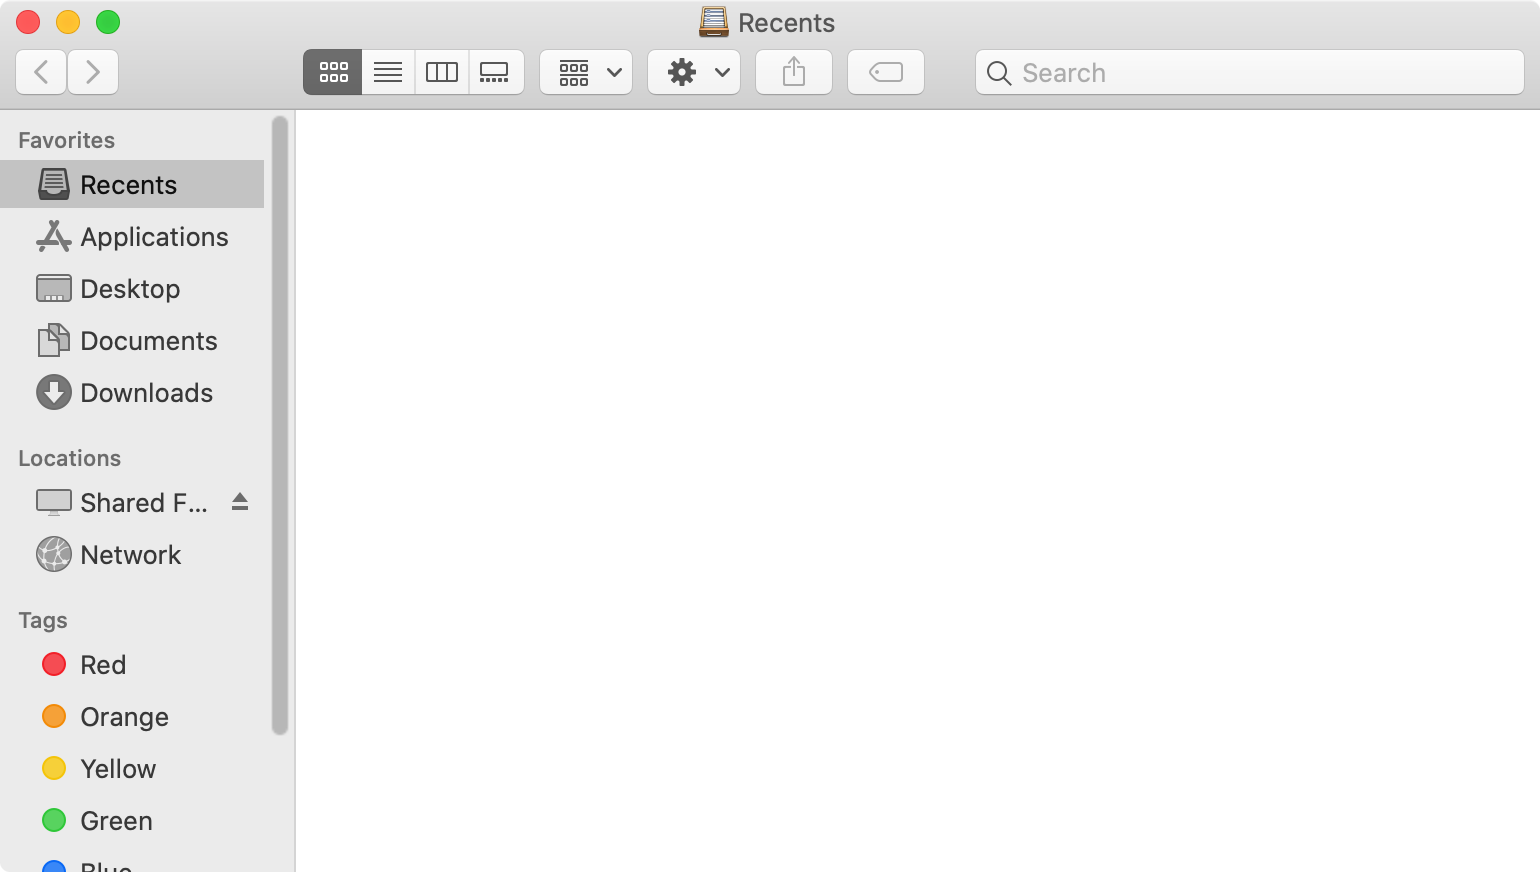
\includegraphics[width=.48\textwidth,clip]{fig/Finder_recents.png}%
    \label{fig:Finder_recents}%
  }\hfill%
  \subfigure[]{%
    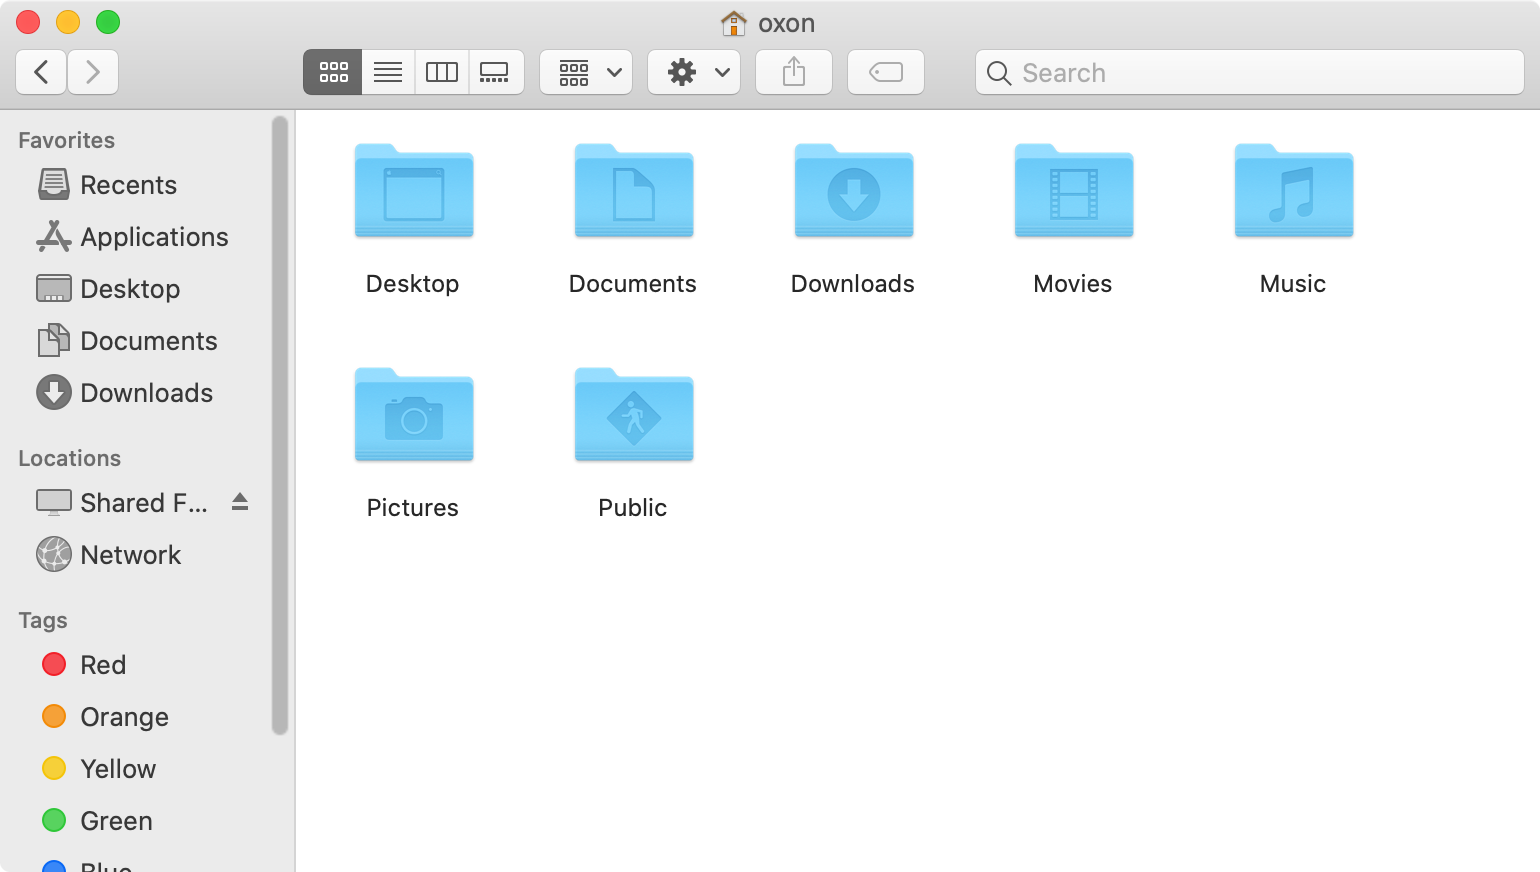
\includegraphics[width=.48\textwidth,clip]{fig/Finder_home.png}%
    \label{fig:Finder_home}%
  }
  \subfigure[]{%
    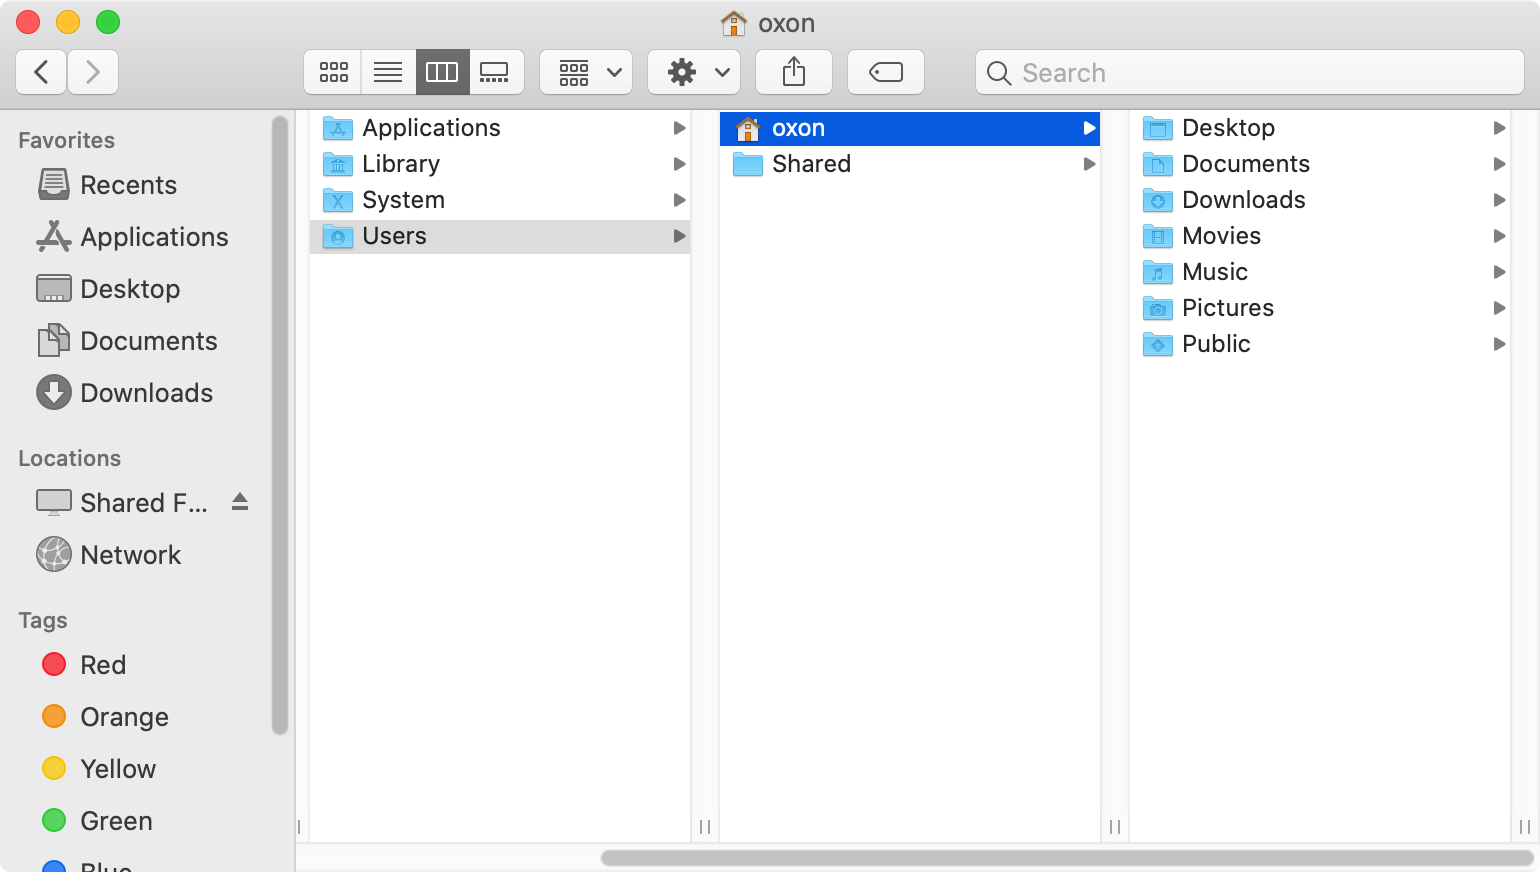
\includegraphics[width=.48\textwidth,clip]{fig/Finder_column.png}%
    \label{fig:Finder_column}
  }\hfill%
  \subfigure[]{%
    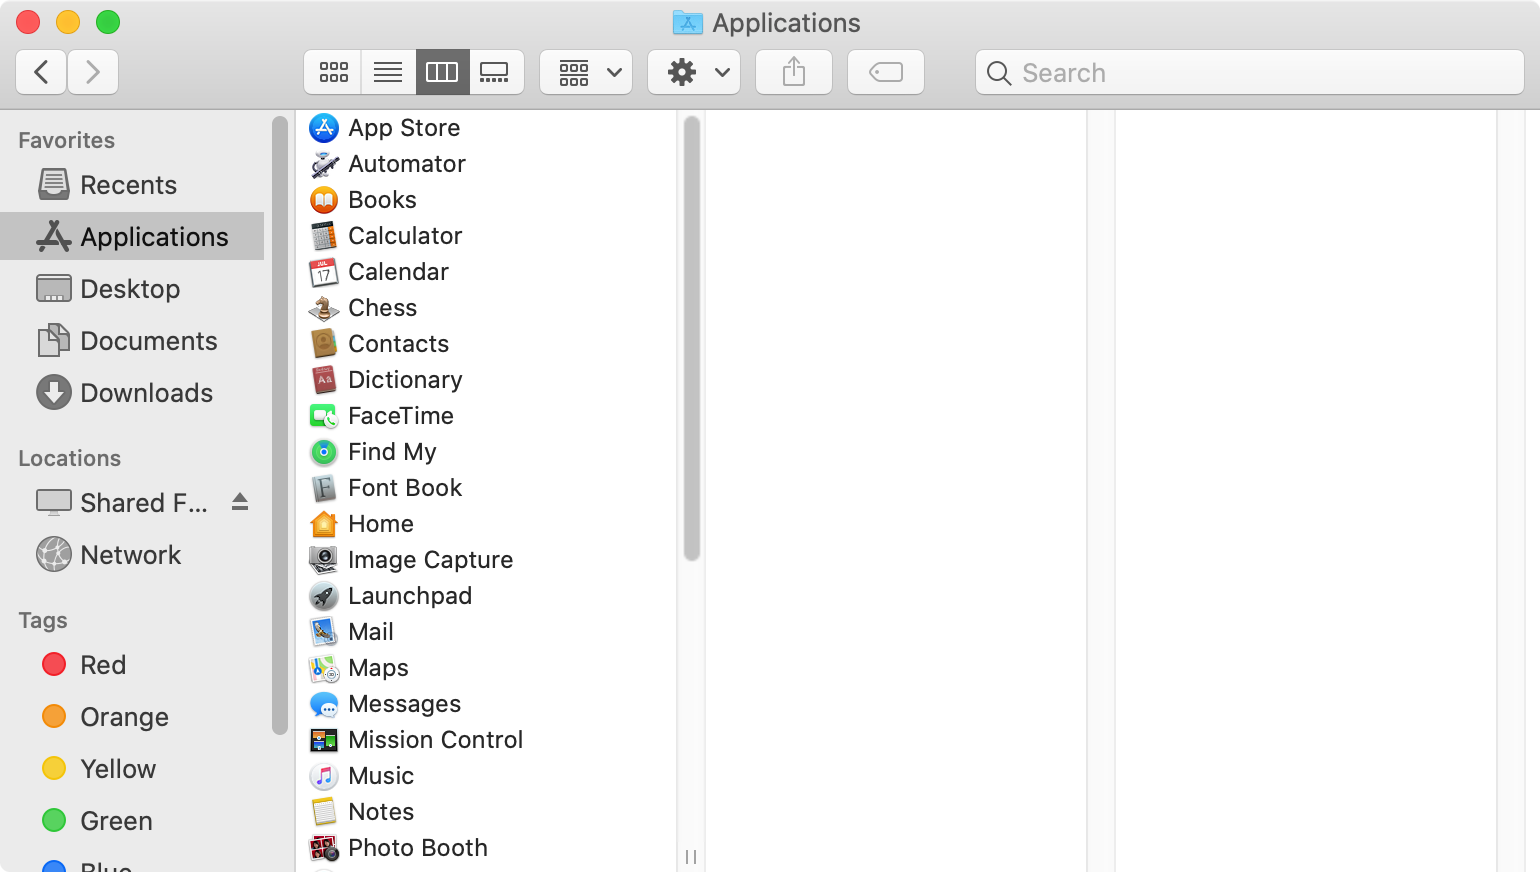
\includegraphics[width=.48\textwidth,clip]{fig/Finder_applications.png}%
    \label{fig:Finder_applications}%
  }
  \caption{Finderの表示例。(a) Recentsの表示。(b)ホームを表示したところ。(c)ホームをカラム表示にしたもの。(d) Applicationsの表示。}
\label{fig:Finder}
\end{figure}

次にシフトキー(Shift)とコマンドキー(\cmdkey\,の記号)とHキーを同時に押すと(\shiftkey\cmdkey\,Hや、Cmd+Shift+Hと表記します)、図~\ref{fig:Finder_home}のようにホーム(Home)に移動します。ホームは個々のユーザが使用できる領域で、実験データや解析プログラムなどは、原則としてホームの下に置きます。アカウント名が例えばoxonの場合、このホームフォルダのパスは\texttt{/Users/oxon}です。

キーボードから複数のキーの組み合わせで、ある特定の動作をさせるものを、キーボードショートカット(keyboard shortcut)と呼びます。Windowsではコントロールキー(Control key)中心ですが、Macの場合はコマンドキー(Command key、\cmdkey)が中心です。例えばコピーやペーストなどのショートカットは、\cmdkey\,Cと\cmdkey\,Vです。

通常、ショートカットはメニューバーから辿ることもできます。既に行ったホームへの移動は、メニューバーの「Go」から「Home」選択すると同じ動作をします。メニューの中にある文字列の右側にショートカットが記載されており、コマンドキー(\cmdkey)、シフトキー(\shiftkey)、オプションキー(\optkey)、コントロールキー(\ctlkey)、デリートキー(\delkey)などと組み合わされたものが表示されています。

さて、Finderの表示がこのままだと移動が不便なので、\cmdkey\,3を押してみましょう。これで表示形式がカラム(column)表示に切り替わります。アイコンが小さくなり情報量が増え、ディレクトリ階層のどこにいるかも分かりやすくなります。

図~\ref{fig:Catalina}のデスクトップ(desktop)\footnote{グラフィカルな画面を持つパーソナルコンピュータが登場した1980年代、その概念を分かりやすくするため机を連想させる用語が導入されました。デスクトップとは机の上であり、そこに様々な書類が置かれたり、また複数の書類をまとめてしまっておくためにフォルダという言葉が使われました。}はデスクトップピクチャ(desktop picture)\footnote{Macでは「壁紙」という言葉ではなくデスクトップピクチャと呼ぶのが正統です。壁紙やwallpaperという言葉は、Windows由来です(窓と壁という連想)。}が表示されているだけで、ファイルは置かれていません。しかしこのデスクトップもフォルダのひとつになっていて、何かしらのファイルをデスクトップに置くと、図~\ref{fig:Finder_column}に表示されているDesktop(\texttt{/Users/oxon/Desktop})にそのファイルが表示されます。試しに\cmdkey\,\shiftkey\,3を押してみてください。これでスクリーンショット(screenshot)が撮影され、デスクトップにPNG画像として保存されるはずです。

次に、\cmdkey\,\shiftkey\,Aを押してみてください。図~\ref{fig:Finder_applications}に表示が切り替わるはずです。macOSにインストールされるアプリケーションの多くはこのApplicationsフォルダ(\texttt{/Applications})に配置されます。ただし、Finderのようにシステムに非常に近い動作をするような一部のアプリケーションは、ここには置かれていません。

\subsection{System Preferences}
System PreferencesはユーザがMacの設定を好みに変更するためのアプリケーションです。日本語環境では「システム環境設定」と呼ばれます。起動すると図~\ref{fig:SystemPreferences}が開き、様々な設定項目を変更することができます。
\begin{figure}
  \centering
  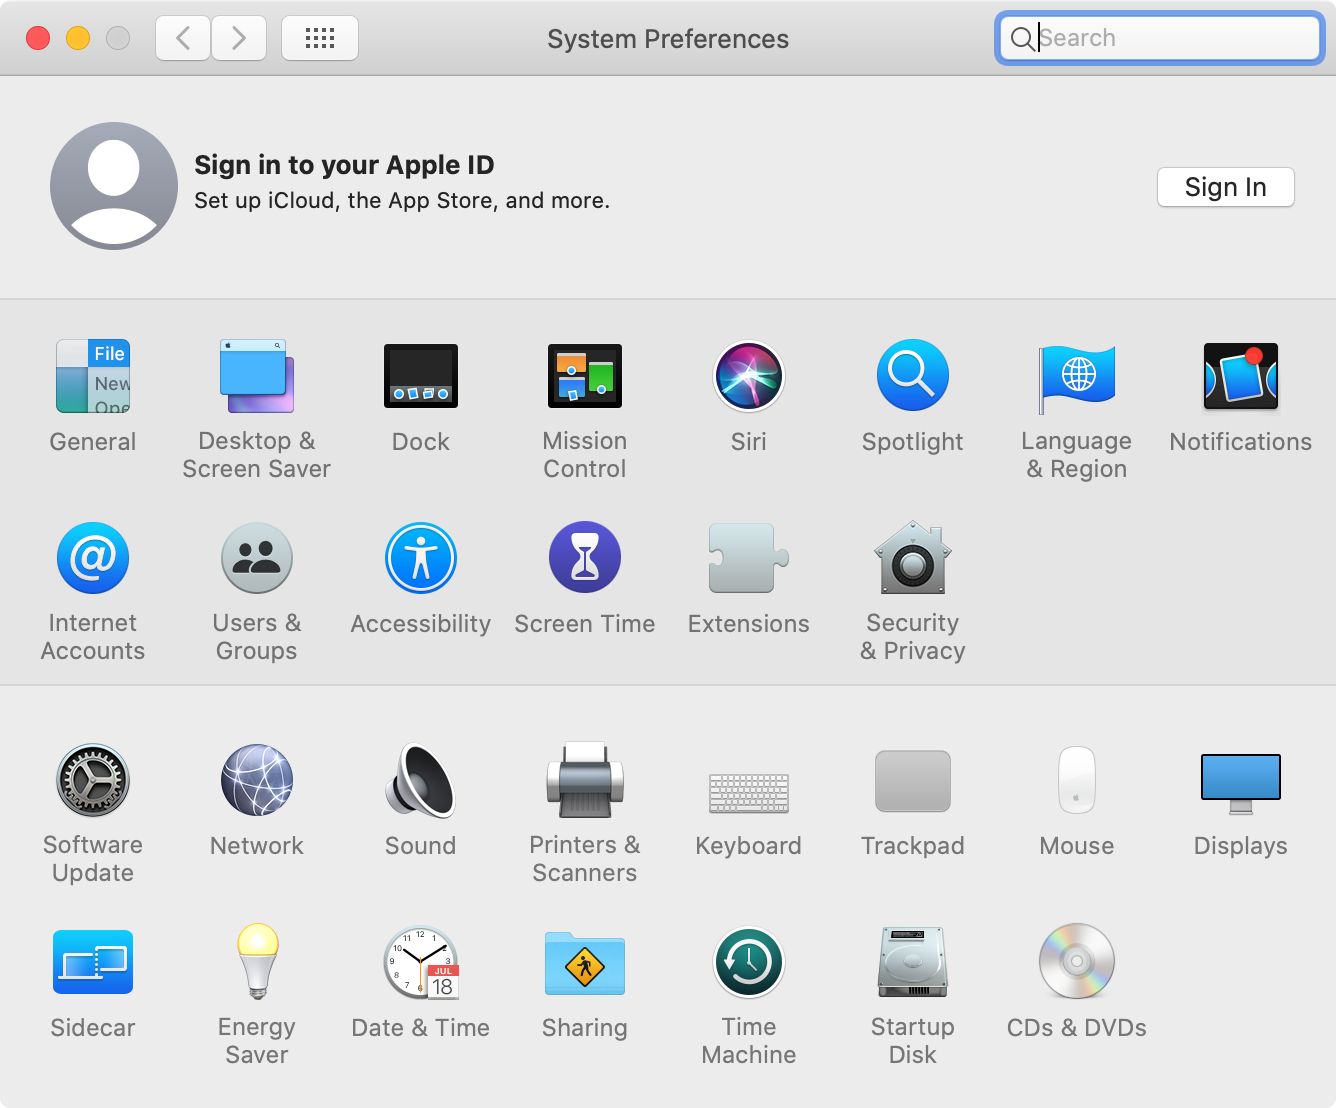
\includegraphics[scale=0.35]{fig/SystemPreferences.png}
  \caption{System Preferencesの画面}
  \label{fig:SystemPreferences}
\end{figure}

\subsection{Safari}
SafariはmacOS、iOS(iPhone)、iPadOS(iPad)に搭載されている、標準のウェブブラウザ(web browser)です。通常の使用であればSafariでも問題ありませんが、より機能拡張したい、WindowsやLinuxと同じ環境に揃えたいという場合は、Google Chromeなど他社製のブラウザを追加インストールすることもできます。

Safariを使用してROOTなどのファイルをインターネットからダウンロードした場合、図~\ref{fig:Finder_column}に表示されているDownloadsフォルダ(\texttt{/Users/oxon/Downloads})に保存されます。
\subsection{Mail}
MailはmacOS標準の電子メールクライアント(E-mail client)\footnote{クライアントとは、サーバと情報のやり取りをするソフトウェアを指すコンピュータ用語です。}です。WindowsやLinuxと環境を揃えたい場合は、Thunderbirdなど他社製のクライアントを追加インストールすることもできます。電子メールクライアントは比較的枯れた技術ですので、特に強い好みがない場合は、Mailを使っておけば十分だと思います。

Mailは一般名詞であり、会話中でも文章中でも一般名詞との区別が困難なことから、Mail.appやApple Mailと呼ぶことが頻繁にあります。ここで、\texttt{.app}はmacOSでアプリケーションに使われる拡張子です。

\subsection{Spotlight}
Dockに表示されているアプリケーション以外にも、\ref{subsec:Finder}~節で説明したように\texttt{/Applications}に多くのアプリケーションがあります。このようなアプリケーションをクリックで起動したりするのは面倒です。そこで、macOS標準の検索機能であるSpotlightを使用してみましょう。

\cmdkey\,Spaceを押してみてください\footnote{図~\ref{fig:Catalina}にあるSpotlightのアイコンをクリックするのでも同じように機能します。}。図~\ref{fig:Spotlight}が現れ、そこに例えば「Finder」と入力すると、図~\ref{fig:Spotlight_results}のように検索結果が現れます。ここでリターンキー(\returnkey)を押すと、Finderを開こうとするため、Finderがアクティブの状態(全てのアプリケーションよりも手前に来る状態)になります。また\cmdkey\,\returnkey\,を押すと、その項目をFinder上で表示します。Finder.appの実体が\texttt{/System/Library/CoreServices/}にあることが分かります。

\begin{figure}
  \centering
  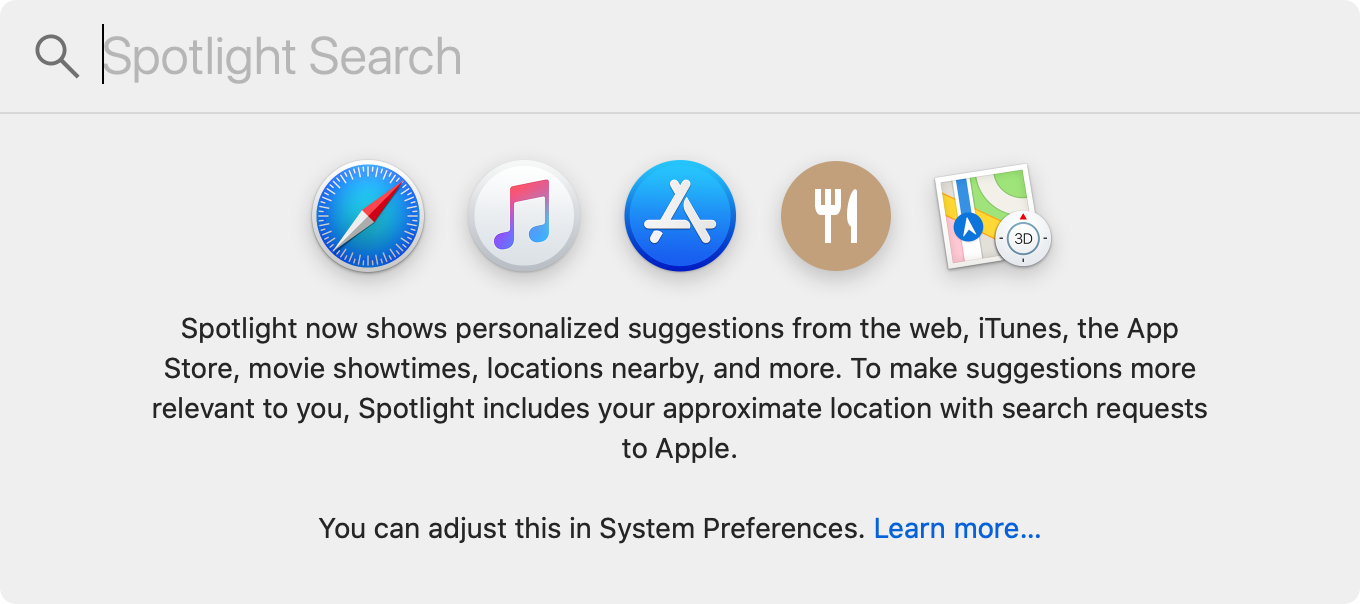
\includegraphics[scale=0.35]{fig/Spotlight.png}
  \caption{Spotlightの画面}
  \label{fig:Spotlight}
\end{figure}
\begin{figure}
  \centering
  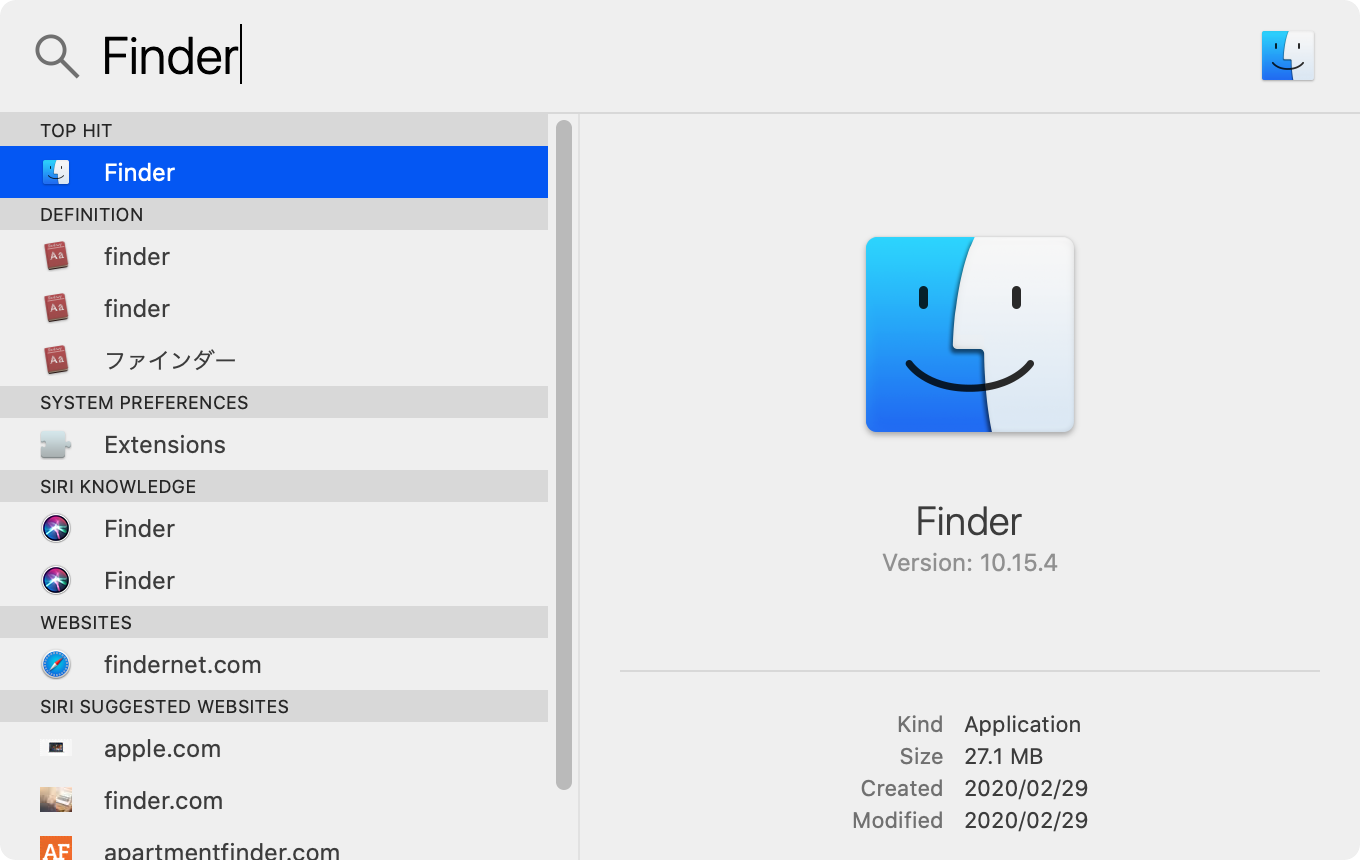
\includegraphics[scale=0.35]{fig/Spotlight_results.png}
  \caption{Spotlightの検索結果の例}
  \label{fig:Spotlight_results}
\end{figure}

\subsection{App Store}
macOSに新しくソフトウェアをインストールするには、大別して4つの方法があります。App Storeを利用する方法(Keynoteなど)、インターネット上でApp Store以外の場所からアプリケーション本体やインストーラをダウンロードしてくる方法(Google Chromeなど)、Homebrewなどのパッケージ管理システムを使用する方法(Pythonなど)、ソースコードをダウンロードして自分でビルドする方法(ROOTなど)です。

macOSのApp Storeは、iPhoneやiPadのApp Store、Android端末上でのGoogle Play、WindowsのMicrosoft Storeと同様のものです。無料のものも有料のものも、次節で説明するApple IDを使用することでインストールすることができます。Microsoft Officeに相当するApple製のPages、Keynote、Numbersなども、このApp Storeからインストールします。

\subsection{Apple IDとiCloud}

App Storeでアプリケーションをインストールする場合、有料・無料を問わずApple IDと呼ばれるアカウントを作成する必要があります\footnote{\url{https://support.apple.com/ja-jp/HT204316}を参照。}。有料ソフトウェアを購入する場合は、クレジットカード情報をさらに付与する必要があります。

Apple IDを登録することで、iCloudというAppleの提供するクラウドサービスを使用できるようになります。研究に関係するところでは、例えば複数のMacでのファイルの同期、Apple ID同士を使っての画面共有などが利用できるようになります。

\subsection{Terminal}
ターミナル(Terminal)はプログラミングやデータ解析などをするときに必要となるアプリケーションです。映画やドラマなどでハッカーやクラッカーが黒い画面に向かってキーボードを連打しているのは、ターミナルで作業をしています。Mailと同じくTerminalは一般名詞であり、macOSに限らずターミナル機能を有する環境は多数あるため、macOSのTerminalアプリケーションを指す場合は、Terminal.appと表記する場合があります。

ターミナルとは「端末」のことです。コンピュータ用語で、ユーザが入出力を行うための装置を指します。現在のようにグラフィカルな操作ができなかった昔のコンピュータでは、ターミナルからコンピュータに指示を出し(入力)、その結果(出力)を受け取るという作業をしていました。プログラミングやデータ解析などでは、今でもターミナルを利用したほうが作業効率が良いため、使われ続けています。

Terminal.appはDockには入っておらず、\texttt{/Applications/Utilities/}にあります。Spotlight(\cmdkey\,Space)を使って起動してみましょう。図~\ref{fig:Terminal}のような画面が現れるはずです。
\begin{figure}
  \centering
  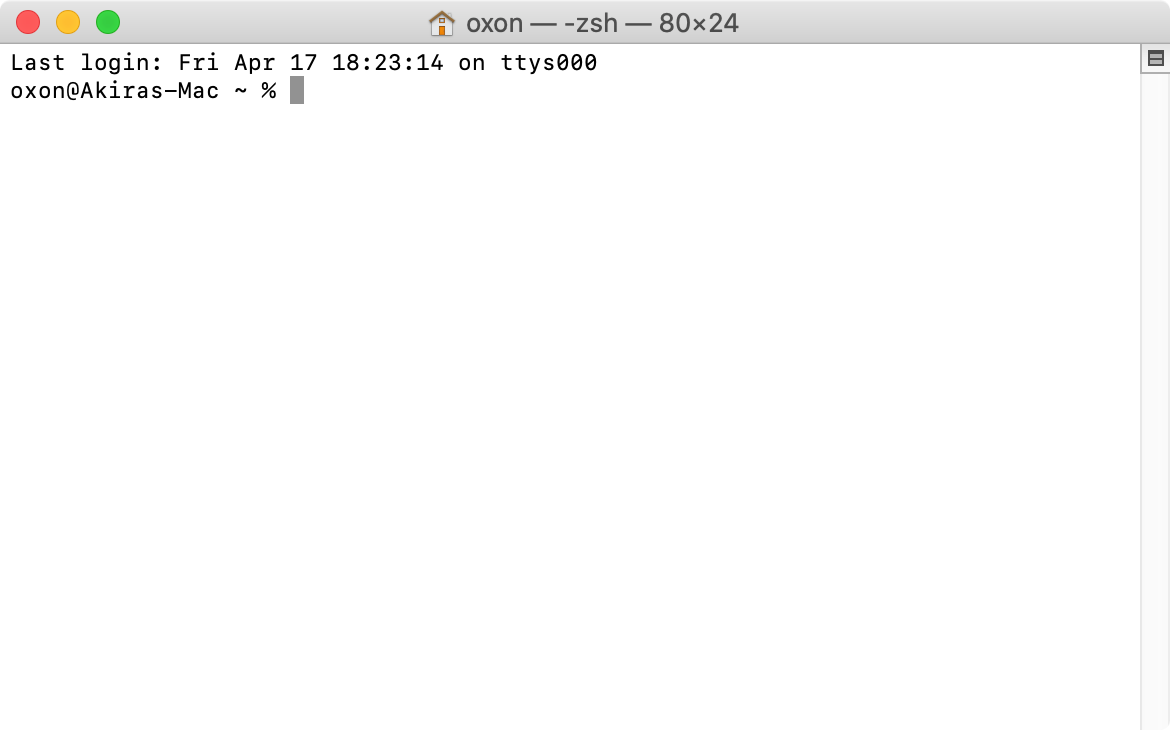
\includegraphics[scale=0.35]{fig/Terminal.png}
  \caption{Terminalの初期画面}
  \label{fig:Terminal}
\end{figure}

\subsection{Time Machine}
Time MachineはmacOSの自動バックアップの仕組みです。設定することで、外付けハードディスクやTime Capsule(タイムカプセル)\footnote{Appleが販売していた、内蔵ハードディスク付きのWi-Fiルータ。}にバックアップを作成することができます。

\subsection{アプリケーションの切り替え}
起動しているアプリケーションを切り替えるのは、\cmdkey\,Tabで行います。同一アプリケーション内でウィンドウを切り替えるのは、\cmdkey\,`で行います。

\section{英語環境にする}
日本の研究室でMacを使う場合、OSの言語環境を日本語にしている人が多いでしょう。しかしMacを研究で使う場合には英語環境に変更することを強くお勧めします。大きく四つの理由があるからです。

まず第一に、インターネット上のMac関係の情報の多くが英語で書かれており、英語で検索した場合に見つかる情報の量と質は日本語の情報を圧倒するからです。使っているMacで何か問題が生じた場合にエラーメッセージが日本語で表示されていると、それを検索語にしても辿り着ける情報には限りがあります\footnote{日本語入力や\LaTeX 関係などの情報だと日本語特有の問題も発生しうるので、そこは臨機応変に対応して下さい。}。Apple社はアメリカの企業でありMacユーザの多くが北米に集中しています。そのためMac関連の情報のやり取りの多くは英語でなされています。これはMacに限らずコンピュータ関係全般に言えます\footnote{恐らく唯一の例外がRubyというプログラミング言語です。これは日本人により開発されたものが世界に広がった希有な例です。}

第二に、あなたは日本人のみと共同研究をするわけではないからです。もしあなたのMacの画面を外国人が見ながら、もしくはあなたが外国人のMacの画面を見ながら作業する時に、OSが英語環境になっていたほうが意志疎通が簡単になることは言うまでもないでしょう。また海外の研究機関などで実験をするときに、現地の実験室で使用するMacやLinuxは英語環境の設定になっていることがほとんどです。様々な国の外国人が実験に参加しているからです。

第三の理由は、ファイル名やメニューの表示が英語になっているほうが作業効率が上がるからです。Macだとホームディレクトリに「書類」や「デスクトップ」というディレクトリが存在しますが、英語環境ではそれぞれ「Documents」と「Desktop」です。Terminal.appからホームで\texttt{ls}すれば、実体が英語名だということがわかります。Finder.appからディレクトリの移動をしたいときに、英語環境であればホームを開いた状態で「do」と連打すれば「Documents」が選択された状態になります。また「de」と打てば「Desktop」が選択されます。例えば図~\ref{fig:Finder_home}の状態で試してみてください。日本語環境の場合だとこうはいきません。またメニューの「編集」は英語環境では「Edit」になっています。メニューで「Edit」を開いた状態で「co」と連打すれば「Copy」のところが選択された状態になるでしょう。

最後の理由は、できる限り英語に慣れ親しんだほうが良いからです。大学院に入りたての頃は、誰しも英語の読み書きと会話に苦労するでしょう。また日本人の多くの研究者はその後何十年も英語で苦労し続けます。少しでも英語に慣れるため、常用するMacくらい英語環境で使う意志を持ちましょう。

ただし、英語環境にすることで問題が生じる場合があります。少し古い話ですが、例えば英語環境でAdobe Flashを表示すると日本語が文字化けすることがありました\footnote{iPhoneやHTML~5の登場によって廃れた技術です。}。他にも英語環境にすると日本語表示がうまくいかないソフトがあるかもしれませんが、そのようなソフトを使うのはやめましょう。日本語表示以外にも色々と問題を抱えている可能性があります。

もし使用しているMacが日本語環境になっている場合、図~\ref{fig:SystemPreferences_language}のように「システム環境設定」から「言語と地域」を開き、「English」を一番上に持ってきてください。これで英語環境に切り替わり、各アプリケーションを起動し直すと英語になります。

\begin{figure}
  \centering
  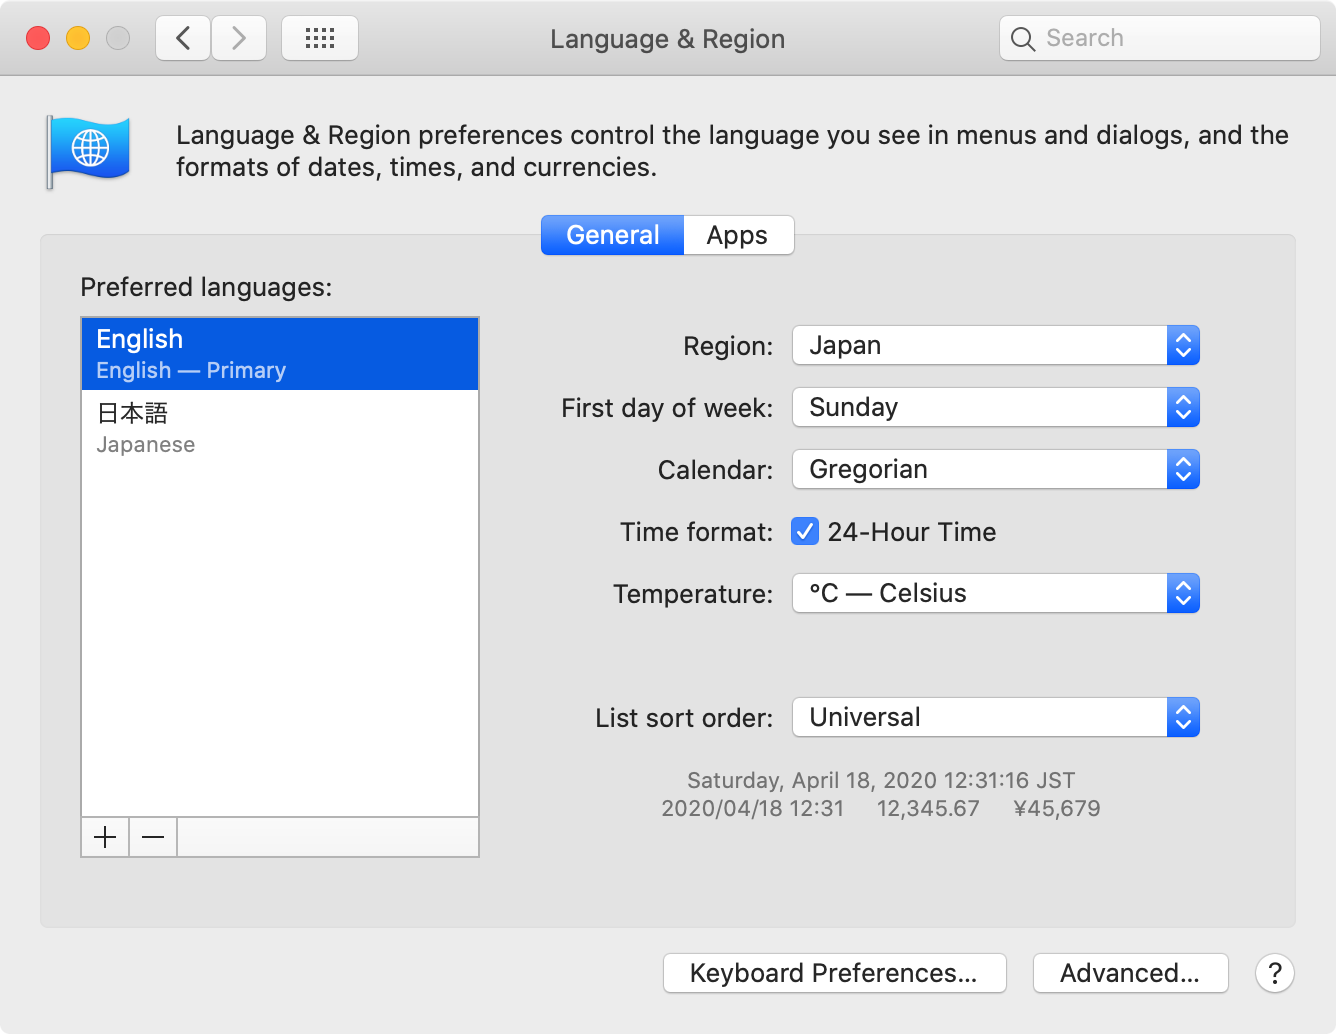
\includegraphics[scale=0.35]{fig/SystemPreferences_language.png}
  \caption{System PreferencesからLanuage \& Region(日本語環境だと「言語と地域」)を開いたところ}
  \label{fig:SystemPreferences_language}
\end{figure}

\section{日本語入力}

もし使用しているMacが既に英語環境になっており、日本語入力ができない状態の場合、図~\ref{fig:SystemPreferences_input}のようにSystem PreferencesからKeyboardを開き、「Input Sources」のところに「Japanese」を追加してください。

\begin{figure}
  \centering
  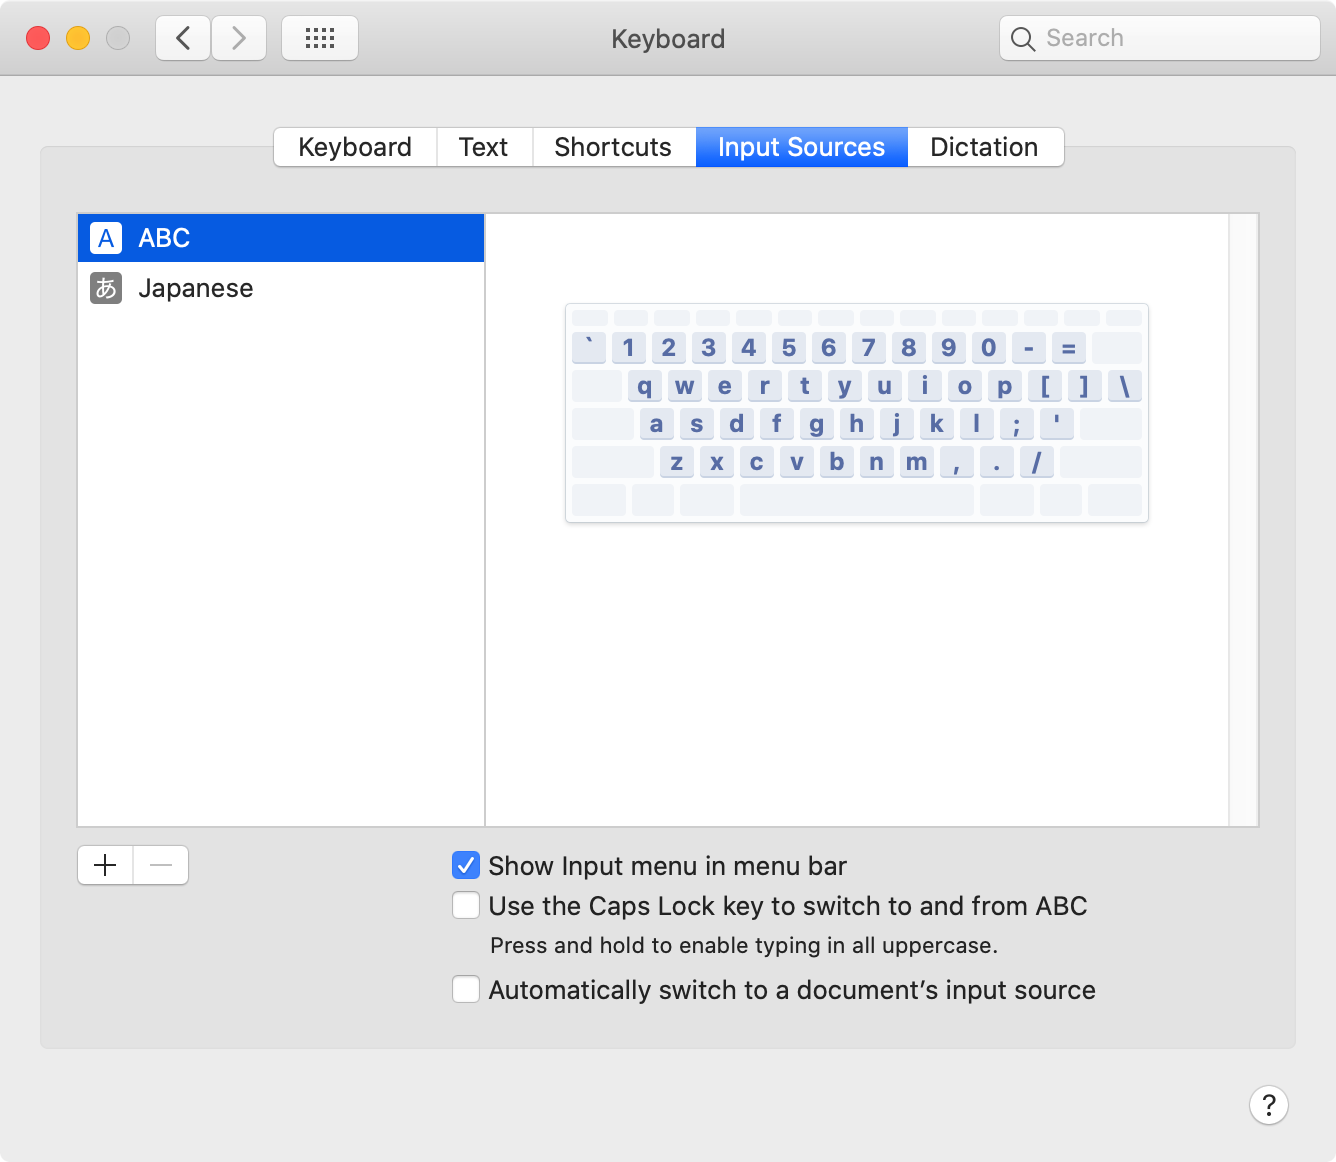
\includegraphics[scale=0.35]{fig/SystemPreferences_input.png}
  \caption{System PreferencesからKeyboardを開いたところ}
  \label{fig:SystemPreferences_input}
\end{figure}

日本語キーボード(JIS配列)のMacを使用している場合、スペースキーの左側に「英数」、右側に「かな」というキーがあるはずです。「英数」を押すと入力が英数に切り替わり、「かな」を押すと日本語入力(ローマ字入力)に切り替わります。もしUSキーボードを使用している場合、\ref{sec:Karabiner}節を参照し、左右のコマンドキーを「英数」と「かな」に割り当ててください。

日本語入力と英語入力を切り替えて使っていると、日本語入力モードのときに英単語を打ってしまったり、英語入力モードのときに日本語を打ってしまうという失敗をすることがあります。このような場合、入力済みの文字をいちいち消去する必要はありません。もし日本語入力モードで英単語を打ってしまったら、「英数」キーを左手の親指で2回素早く叩いてください。これで入力済みの文字がアルファベットに変換され、英語入力モードに切り替わります。逆に、英語入力モードのときに日本語を間違えて打ちかけた場合は、「かな」きーを右手の親指で2回叩いてください。

日本語入力と英語入力の切り替えは\ctlkey\,Spaceでも可能です。しかし、これは\ref{sec:Emacs}~節で後述するショートカットと競合してしまうため、節~\ref{sec:Keyboard}で設定を無効にします。

\section{Finderの設定}
まずはFinderの設定をしましょう。macOSのアプリケーションごと固有の設定は、それぞれのアプリケーションで「Preferences…」というメニューを選択することで行えます。Finderの場合、メニューバーのFinderからPreferences…を選びます。ショートカットは多くのアプリケーションで\cmdkey\,,です。

\begin{figure}
  \centering
  \subfigure[]{
    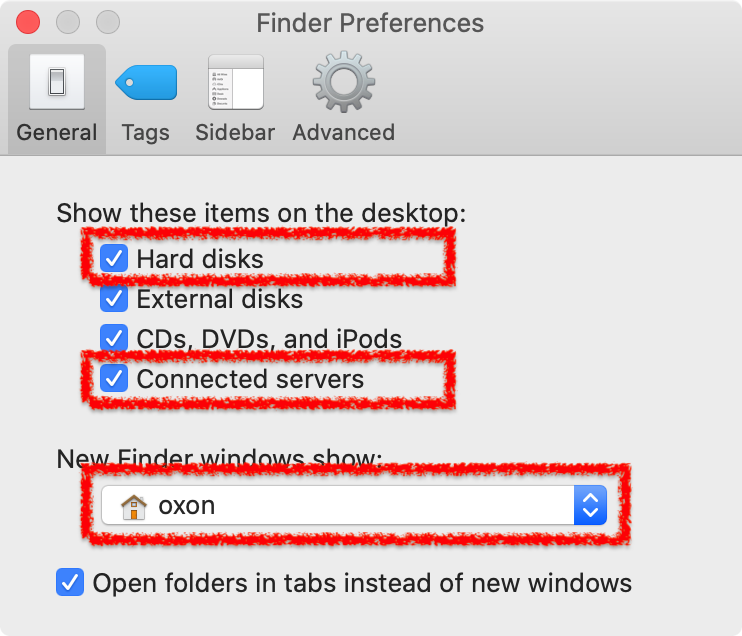
\includegraphics[width=.32\textwidth,clip]{fig/FinderPreferences_general.png}%
    \label{fig:FinderPreferences_general}%
  }\hfill%
  \subfigure[]{%
    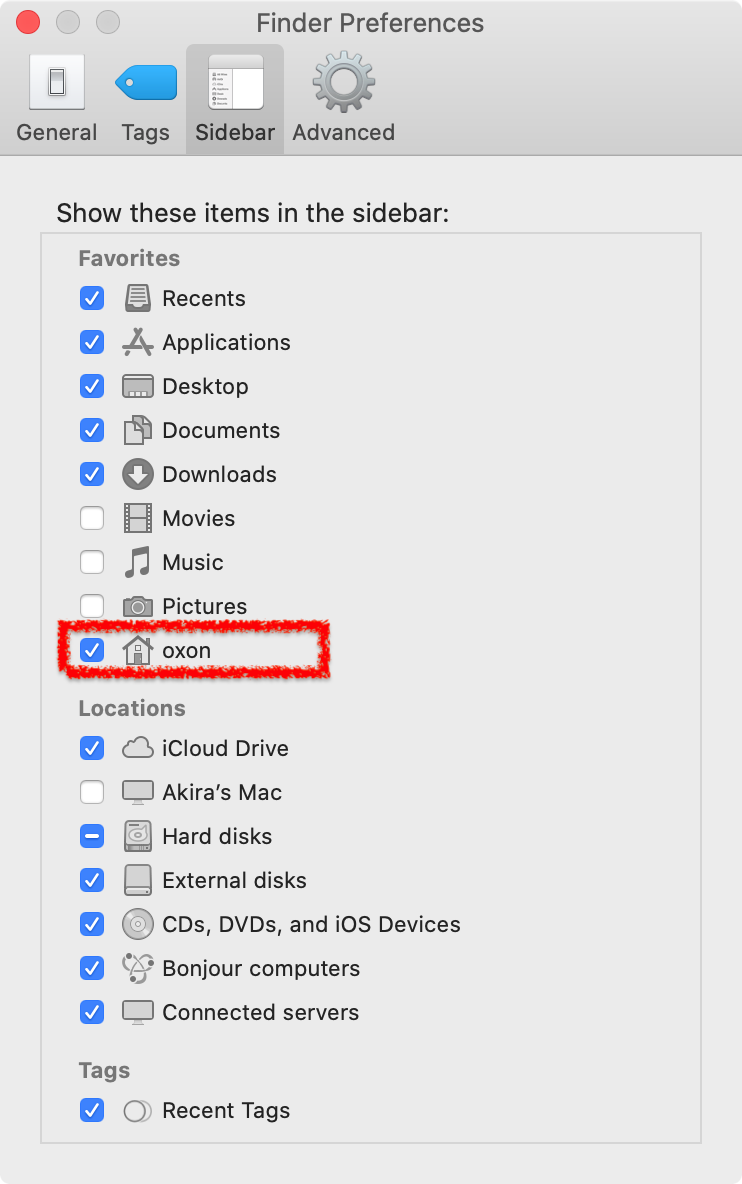
\includegraphics[width=.32\textwidth,clip]{fig/FinderPreferences_sidebar.png}%
    \label{fig:FinderPreferences_sidebar}%
  }\hfill%
  \subfigure[]{%
    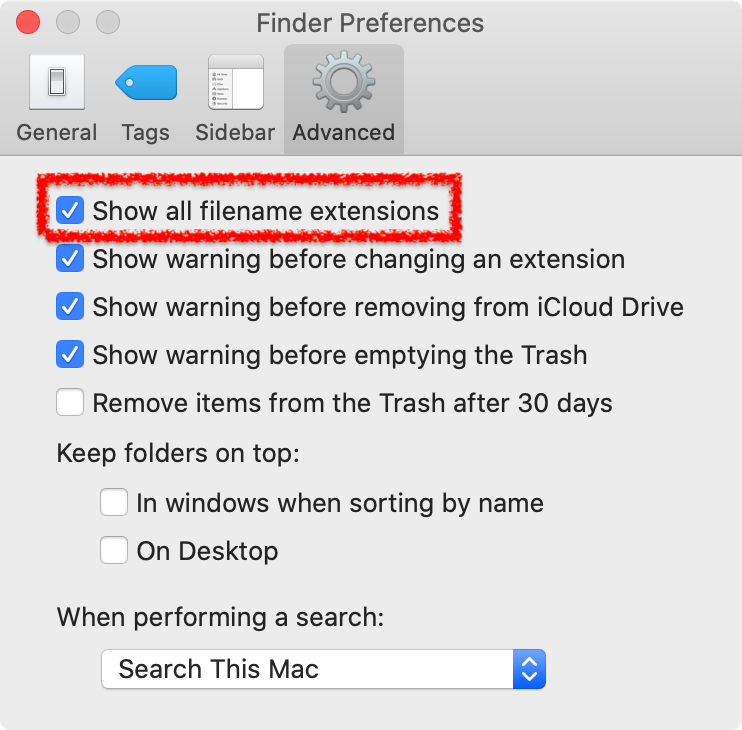
\includegraphics[width=.32\textwidth,clip]{fig/FinderPreferences_advanced.png}%
    \label{fig:FinderPreferences_advanced}
  }
  \caption{Finderの設定}
\label{fig:FinderPreferences}
\end{figure}

まずデスクトップに内蔵ハードディスク(SSD含む)と接続したサーバを表示するように、図~\ref{fig:FinderPreferences_general}を見て「General」のタブから設定を変更します。また新規にウィンドウを開いたときにホームが表示されるようにします。

次にSidebarのタブから図~\ref{fig:FinderPreferences_sidebar}のように表示する項目にホームを追加します。

最後に「Advanced」のタブを開きます。Macの初期設定では、ファイルの拡張子(extension)が表示されませんので、図~\ref{fig:FinderPreferences_general}のように全ての拡張子を表示する設定に変更します。この表示をしないと、Terminal.appから操作するファイル名とFinderから見えるファイル名が一致しない場合があります。

またディレクトリ階層がわかりやすいように、Finderがアクティブな状態で\cmdkey\,/と\cmdkey\,\optkey\,Pをそれぞれ押します。これで図~\ref{fig:Finder_info}のように項目数やパスの表示がされるようになります。

\begin{figure}
  \centering
  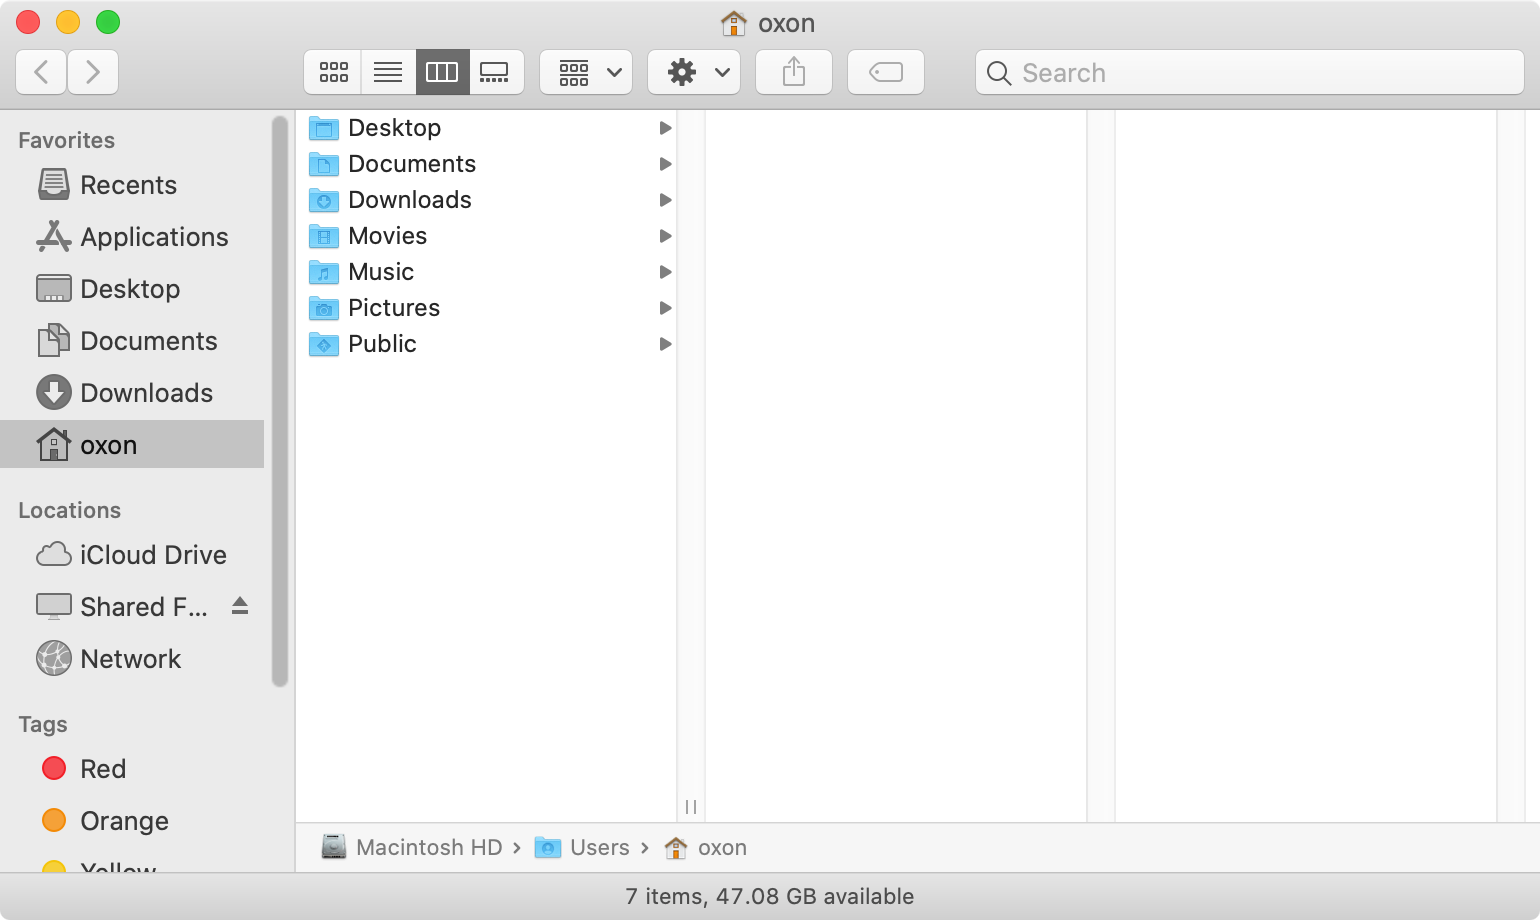
\includegraphics[width=.48\textwidth,clip]{fig/Finder_info.png}
  \caption{Finderの表示を変更した例}
\label{fig:Finder_info}
\end{figure}

\section{キーボードの設定}
\label{sec:Keyboard}

\subsection{Caps LockキーをControlキーに変更する}
もしあなたのMacがUS配列のキーボードならば、Caps LockキーはControlキーとして機能するように設定を変更しましょう。図\ref{fig:Keyboard1}のように、System Preferencesから「Keyboard」を開き「Modifier keys…」を押し、Caps LockをControlにします。\ref{sec:Emacs}~節で後述するように、macOS環境ではEmacsの操作体系に倣ったキーボードショートカットが使われています。そのためControlキーの使用率が他のOSに比べて非常に高くなるのが特徴です。US配列のキーボードを使用している場合にはControlキーが押しにくい位置にあるため、滅多に使わない、かつ最も押しやすい位置にあるCaps LockをControlキーにしてしまうことがよく行われています。

\begin{figure}
  \centering
  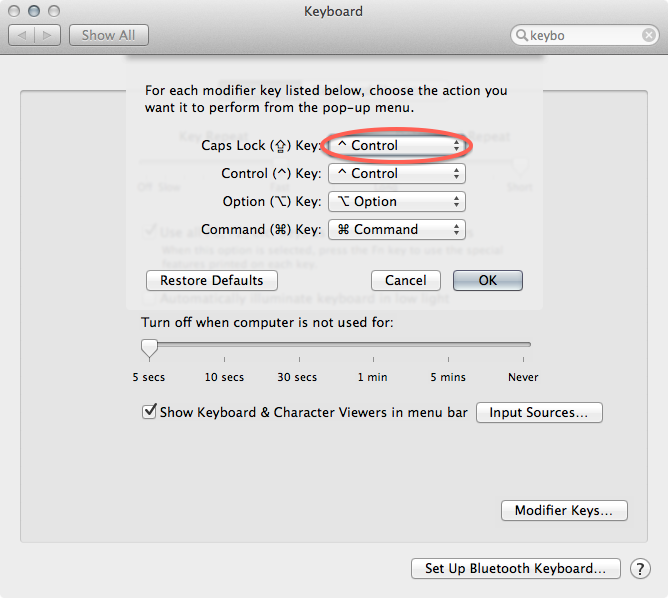
\includegraphics[scale=0.35]{fig/Keyboard1.png}
  \caption{Caps LockをControlキーに変更する}
  \label{fig:Keyboard1}
\end{figure}

\ref{sec:Karabiner}~節で説明するKarabiner-Elementsをインストールする場合、ここでのCaps Lockキーの置き換えはする必要はありません。Karabiner-Elementsで同様の設定を行います。

\subsection{入力切り替えの無効化}
日本語入力と英語入力の切り替えは、デフォルトでは\ctlkey\,Spaceになっています。しかしこれは図\ref{fig:Keyboard2}のように「Shortcuts」タブから無効化します。「英数」キーと「かな」キーから切り替えてください。

\begin{figure}
  \centering
  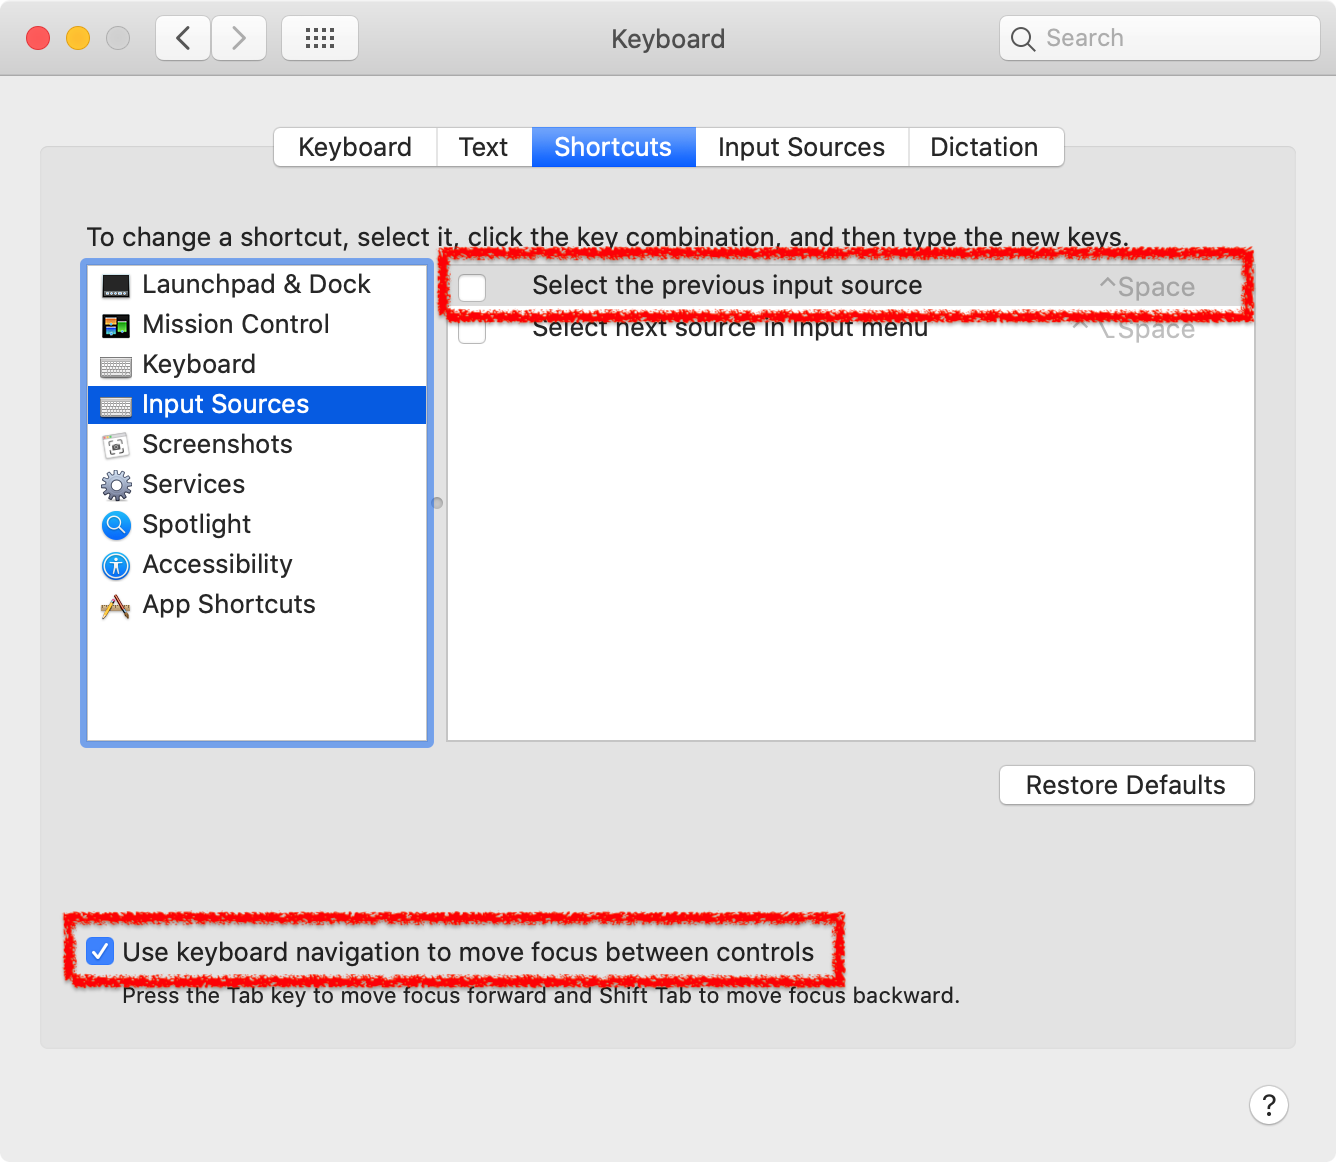
\includegraphics[scale=0.35]{fig/Keyboard2.png}
  \caption{入力の切り替えを無効化し、また全てのボタンなどをTabキーで移動できるようにする}
  \label{fig:Keyboard2}
\end{figure}

\subsection{Tabキーの動作の変更}
次に同じく「Shortcuts」のタブから、図\ref{fig:Keyboard2}のようにボタンなどの選択を全てTabキーで行えるようにします。このようにすることで、様々な画面操作をするときに、いちいちキーボードからトラックパッドやマウスへ手の移動をしなくて済むようになります。

例えばゴミ箱(Trash)を空にする際、図\ref{fig:Trash_Dialog}のような確認ダイアログが出てくるはずです。ここで数回Tabキーを押すと「Cancel」ボタンの強調表示(青線での縁取り)が「Empty Trash」との間で移動します。縁取られているボタンは、いちいちクリックしなくてもSpaceキーを押すと実行されます。また「Empty Trash」のように青く塗りつぶされているボタンは、リターンキーを押すと実行されます。

\begin{figure}
  \centering
  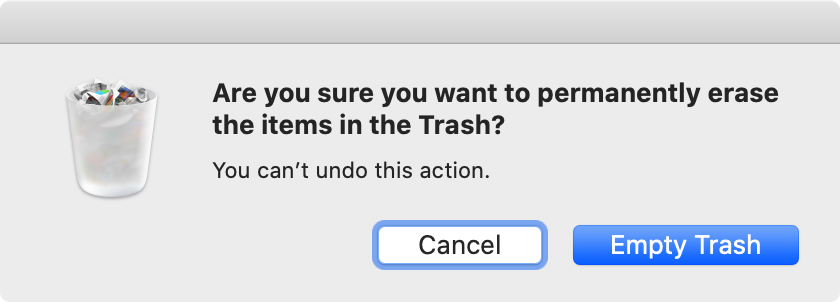
\includegraphics[scale=0.35]{fig/Trash_Dialog.png}
  \caption{ゴミ箱を空にするときのダイアログ}
  \label{fig:Trash_Dialog}
\end{figure}

\subsection{キーボードの繰り返し入力速度}
デフォルトでは、キーボードの繰り返し入力速度は非常に遅い設定になっています。例えばTerminal.appでaキーを押しっぱなしにしても、えらいのんびりと入力されます。図~\ref{fig:Keyboard_speed}のように、キーの繰り返し入力の速度を一番速くしてください。また繰り返し入力が開始されるまでの待ち時間も一番短くしてください。トラックパッド(Trackpad)のカーソル移動速度も、同じようにSystem Preferences のTrackpadのところから最速にしましょう。慣れてください。人生は時間が限られています。

\begin{figure}
  \centering
  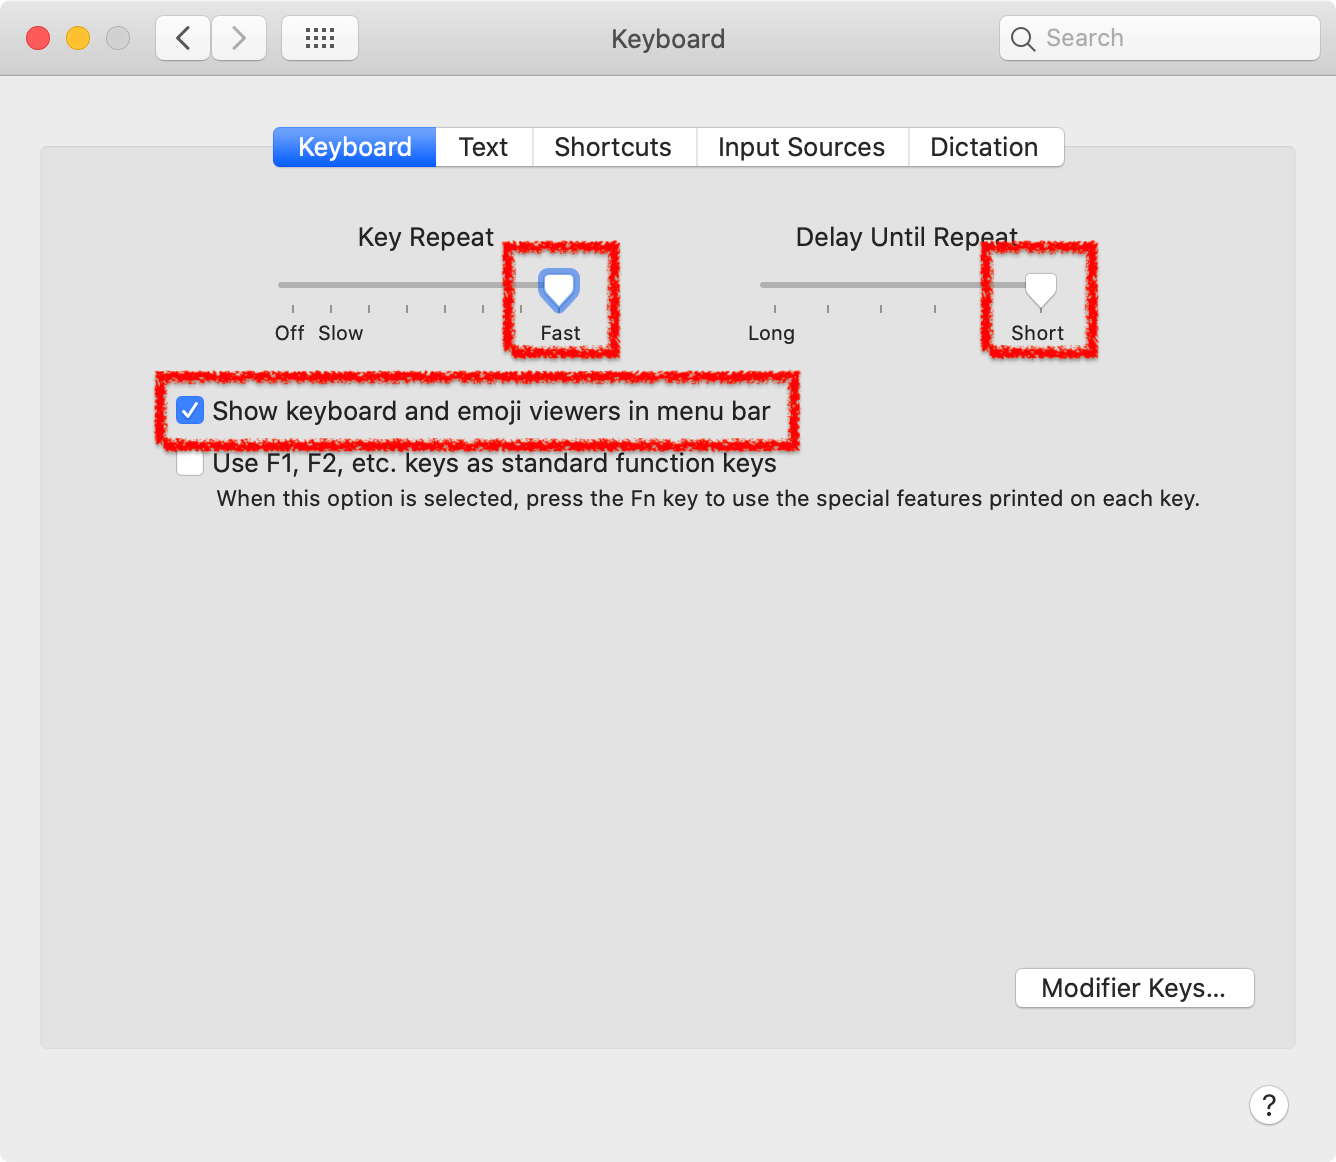
\includegraphics[scale=0.35]{fig/Keyboard_speed.png}
  \caption{繰り返し入力速度の変更}
  \label{fig:Keyboard_speed}
\end{figure}

ついでに、メニューバーの入力メニューのところから、記号や絵文字を探すパネルを表示できるようにしておくと便利です。

\section{Karabiner-Elementsによるキーボードの操作性向上}
\label{sec:Karabiner}

\ref{sec:Emacs}で述べるように、macOSのキーボード操作の多くはEmacsの操作体系に基づいています。しかし、この操作に対応していないアプリケーションも存在するため(Microsoft製品やAdobe製品など)、Karabiner-Elements\footnote{\url{https://karabiner-elements.pqrs.org}}をインストールすることでmacOSの操作を快適にすることができます。

他のmacOSアプリケーションのインストールでも同様の手順を踏むことがあるため、ここではKarabiner-Elementsを例として、インストール方法を簡単に説明します。

まずKarabiner-Elementsのウェブサイトから、ディスクイメージをダウンロードします\footnote{ディスクイメージ(disk image)とはmacOSのファイル形式のひとつで、マウント可能なボリューム(例えばUSBメモリなど)のように取り扱えるものです。拡張子は\texttt{.dmg}です。}。図~\ref{fig:Karabiner_download}のように、ダウンロードしたファイルはSafariのDownloadsの一覧に表示され、また\texttt{\~{}/Downloads}の中に保存されることが分かります。

\begin{figure}
  \centering
  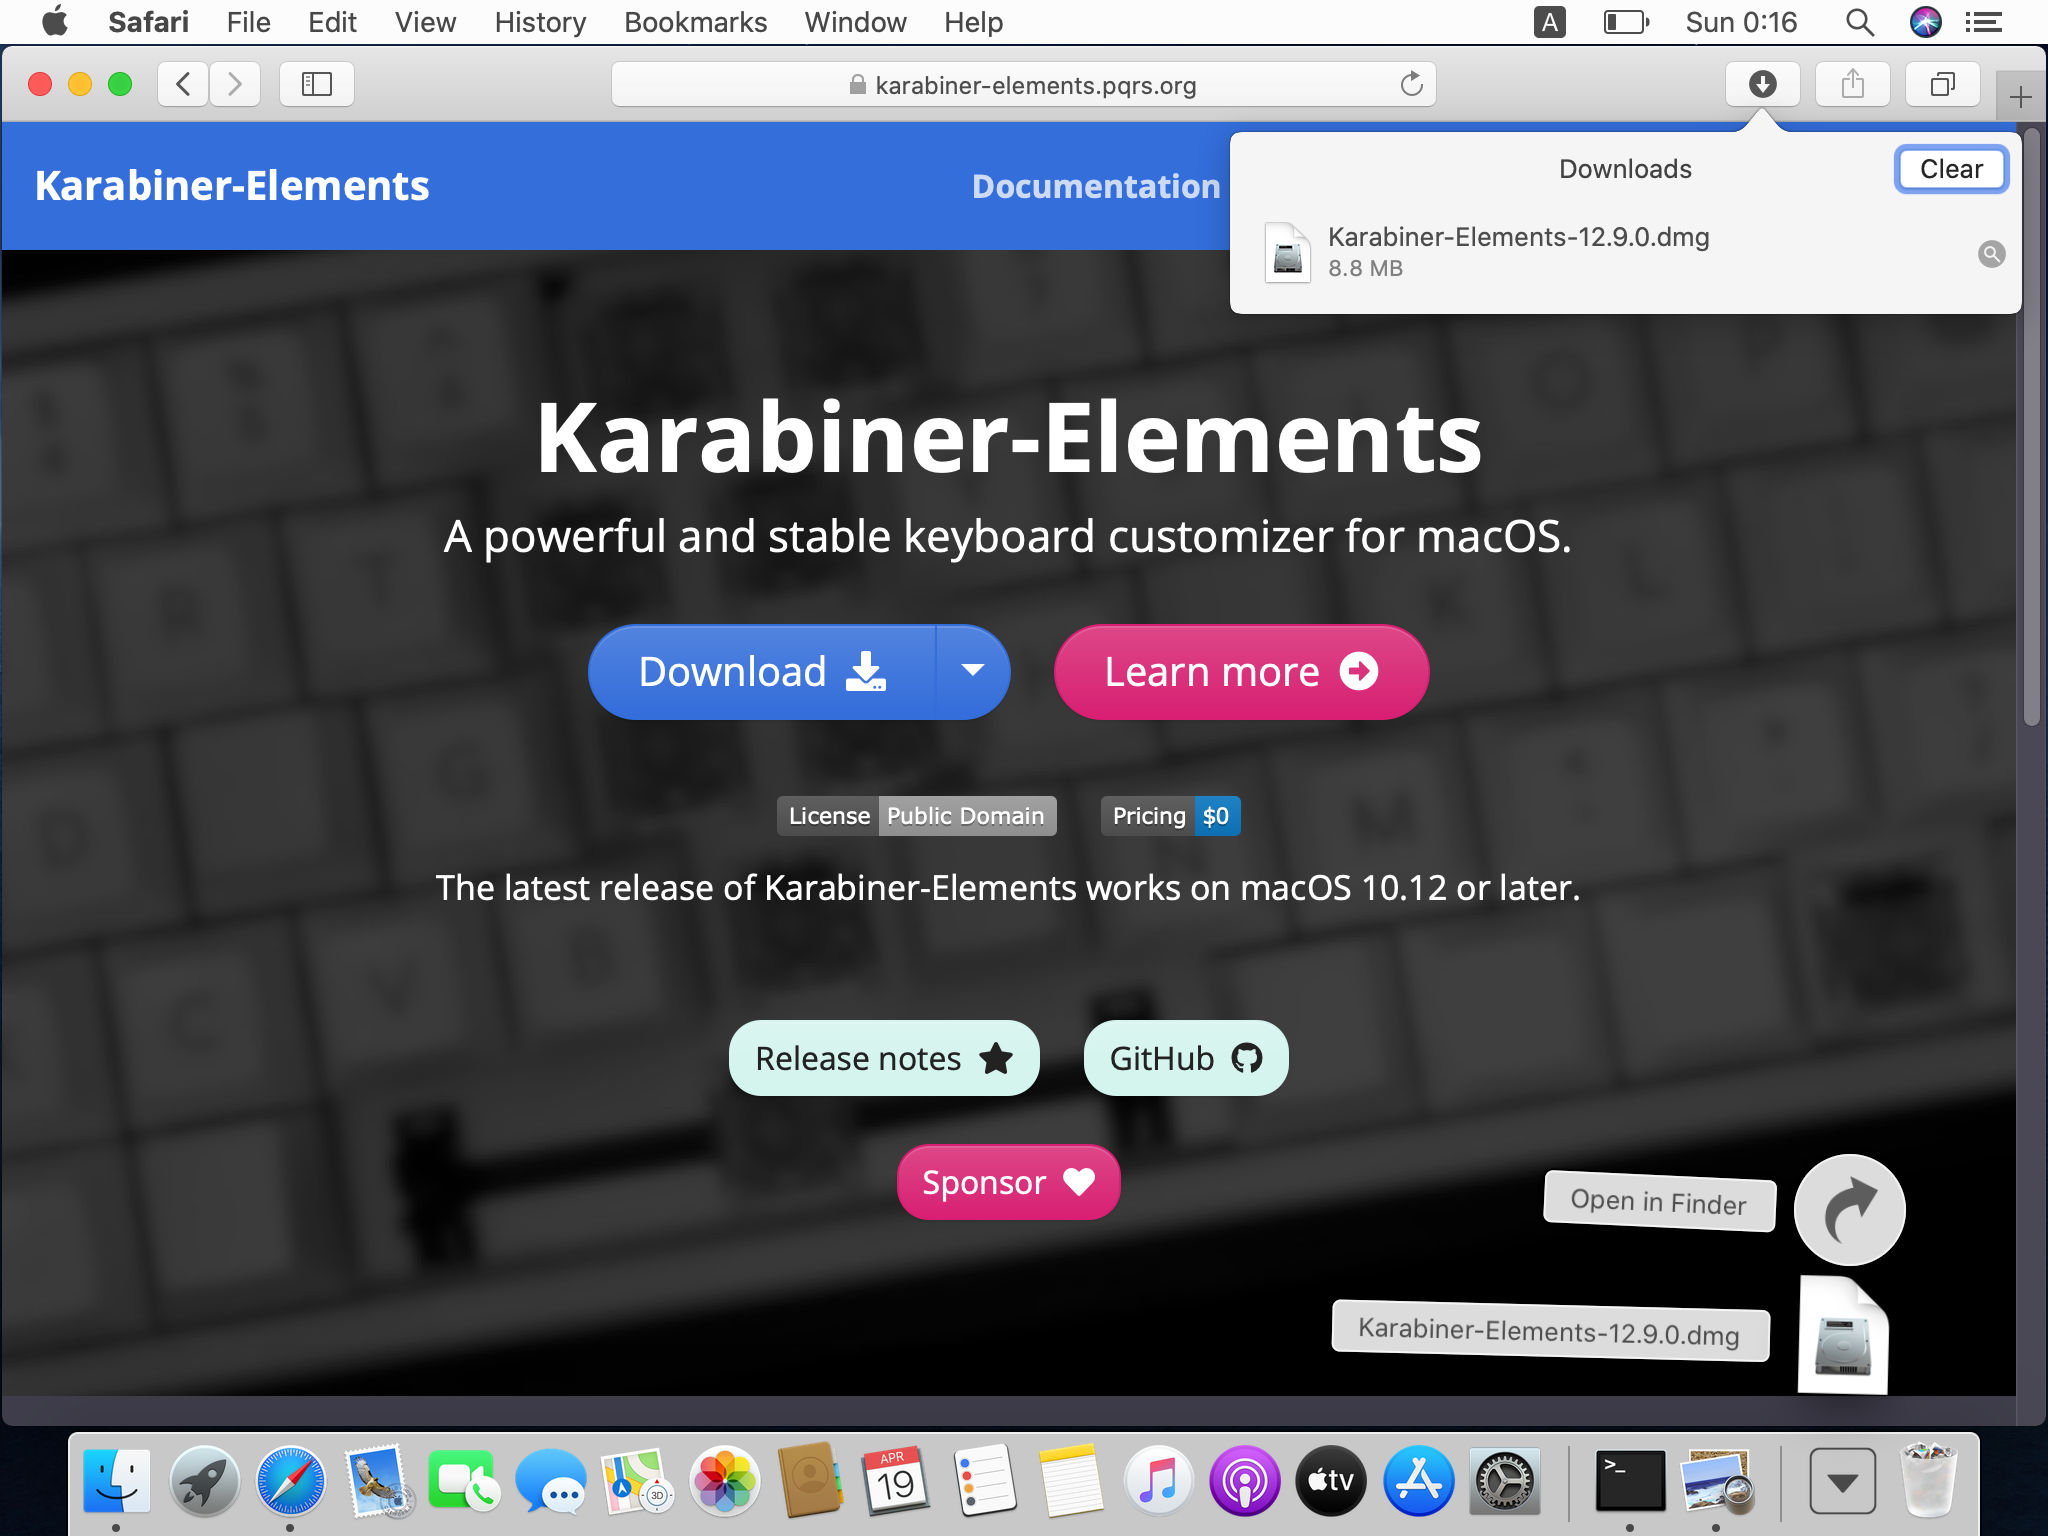
\includegraphics[scale=0.35]{fig/Karabiner_download.png}
  \caption{Karabiner-Elementsのダウンロード}
  \label{fig:Karabiner_download}
\end{figure}

このディスクイメージを開くと仮想的にマウントされ、デスクトップ上にマウント済みのボリュームが表示されます。この中に、パッケージファイル\footnote{パッケージファイル(package file)とは、macOSで複数のフォルダやファイルから構成されるものを擬似的に単一ファイルのように表示しているものです。拡張子は\texttt{.pkg}です。}が図~\ref{fig:Karabiner_pkg}のように存在します。これがインストーラーです。

\begin{figure}
  \centering
  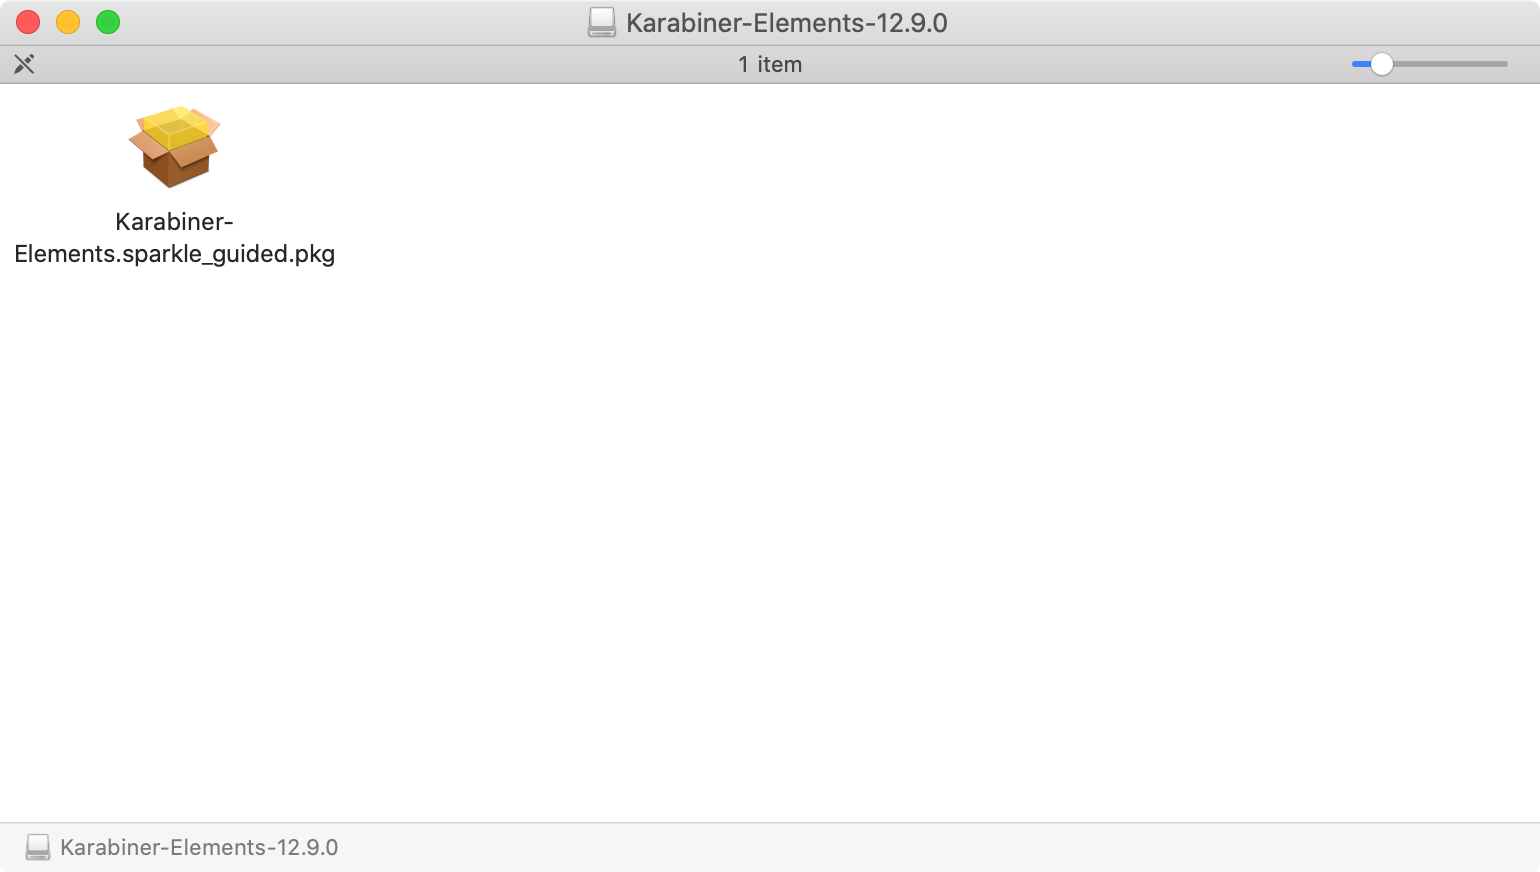
\includegraphics[scale=0.35]{fig/Karabiner_pkg.png}
  \caption{Karabiner-Elementsのインストールパッケージ}
  \label{fig:Karabiner_pkg}
\end{figure}

インストーラーを起動すると、図~\ref{fig:Karabiner_install}のようにmacOSの標準的なインストール画面が表示されます。表示される手順にしたがってインストールしてください。公式の説明は\url{https://karabiner-elements.pqrs.org/docs/getting-started/installation/}にあります。

\begin{figure}
  \centering
  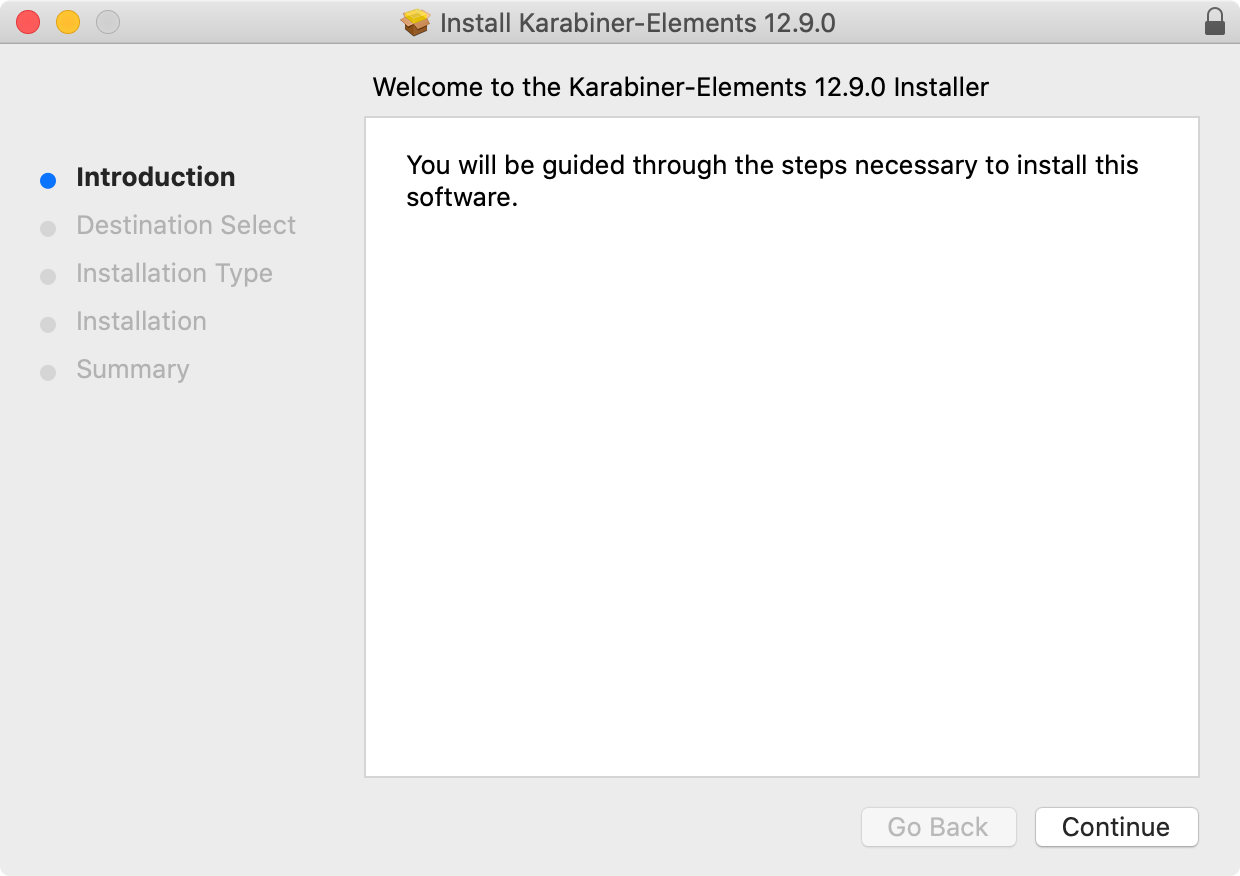
\includegraphics[scale=0.35]{fig/Karabiner_install.png}
  \caption{Karabiner-Elementsのインストール画面}
  \label{fig:Karabiner_install}
\end{figure}

このインストールを進めると、図~\ref{fig:Karabiner_blocked}のような警告が表示されます。これは、App Storeなどの認証を経ていないソフトウェアをインストールしたり起動したりする場合などに表示されます。コンピュータウイルスのように悪意の持ったプログラムを実行するときもこのような警告が出るはずですので、インストールしようとしているにはソフトウェアが怪しいものでないか、よく注意してください。

\begin{figure}
  \centering
  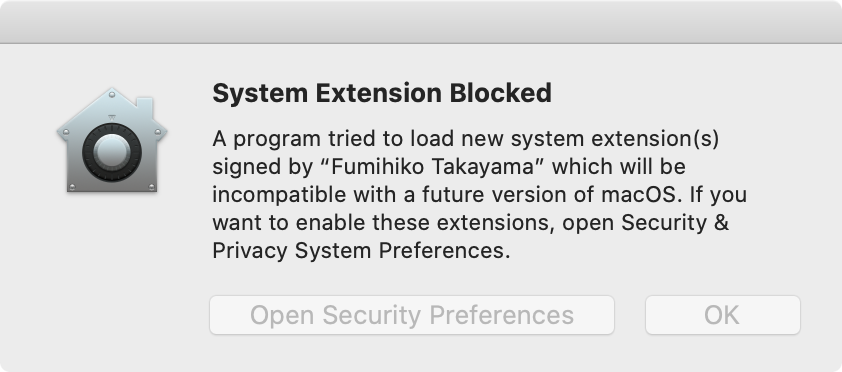
\includegraphics[scale=0.35]{fig/Karabiner_blocked.png}
  \caption{Karabiner-Elementsの警告}
  \label{fig:Karabiner_blocked}
\end{figure}

この警告ではインストールしようとしている機能拡張(System Extension)がブロックされたと書かれています。これを解除するためには、指示に従い、System Preferences の Security \& Privacy を開いてください。

そうすると、図~\ref{fig:Karabiner_allow}のような画面になっているはずです。まず左下の鍵アイコンをクリックして管理者権限で解錠します。このように管理者権限が必要となるOSの設定変更は、この鍵アイコンをその都度クリックする必要があります。解錠するとブロックされたソフトウェアを許可するためのAllowボタンが押せるようになります。今回の場合、Karabiner-Elementsとその開発者である Fuihiko Takayama 氏は信頼できますので、Allowを押してください。これで、Karabiner-Elementsのインストール作業は終わりです。

\begin{figure}
  \centering
  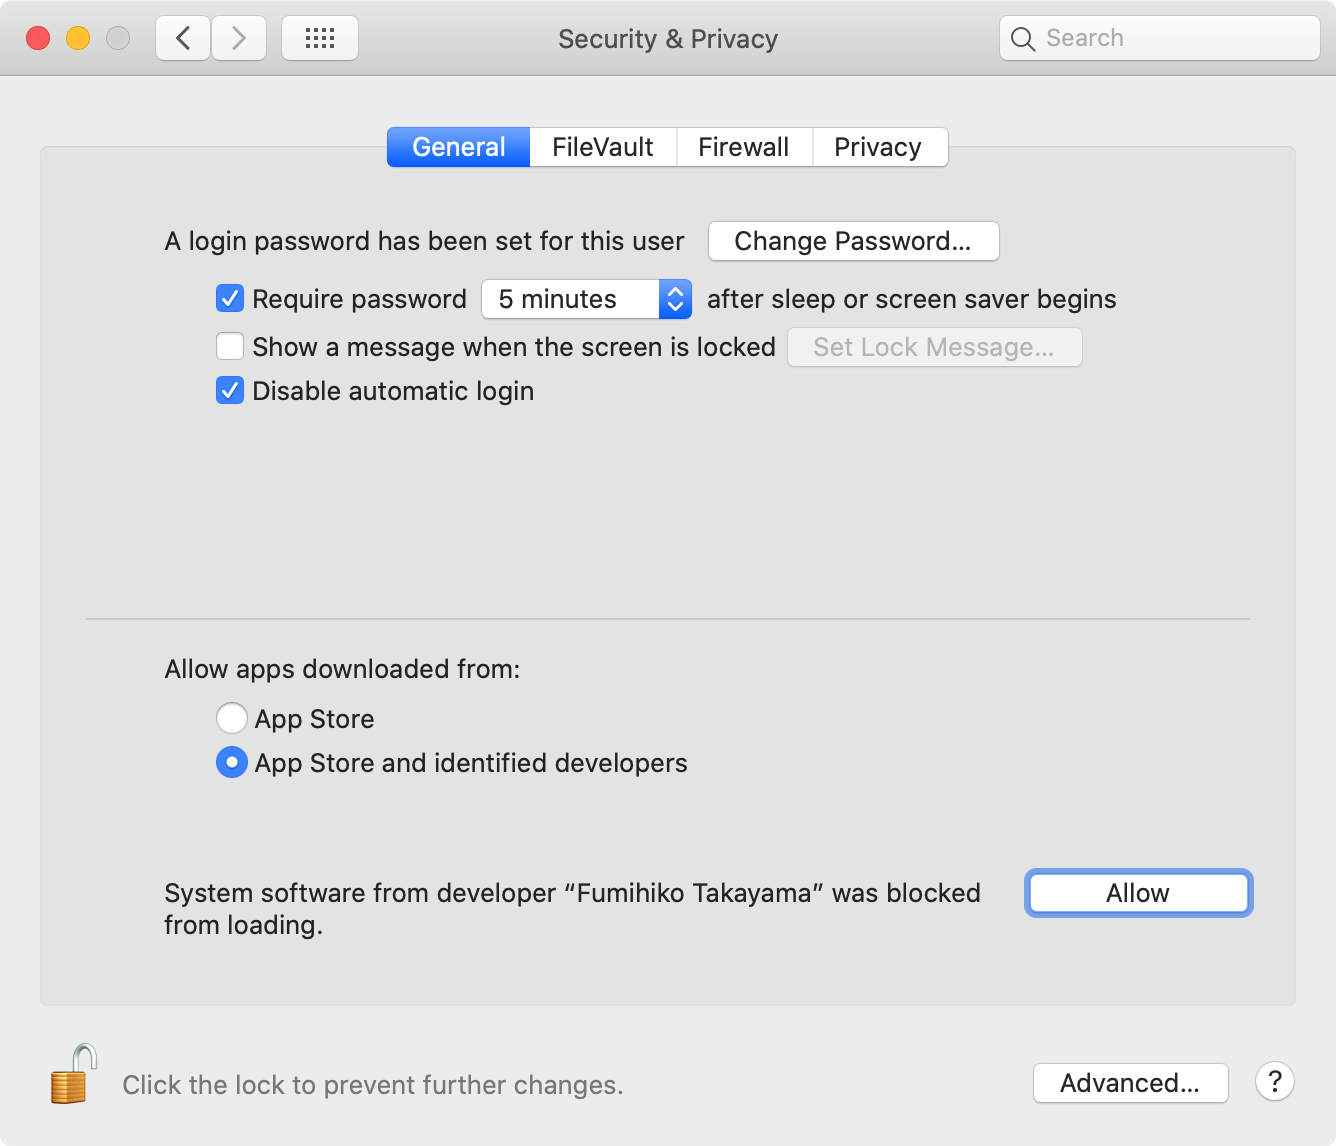
\includegraphics[scale=0.35]{fig/Karabiner_allow.png}
  \caption{Karabiner-Elementsの許可}
  \label{fig:Karabiner_allow}
\end{figure}

Karabiner-Elementsをインストール後、SpotlightからKarabiner-Elements.appを起動してください。そうすると、まず最初に図~\ref{fig:Karabiner_keystroke}のように許可を求めるダイアログが出るはずです。このようなダイアログは、一部のアプリケーションの初回起動時に現れることが頻繁にあります。Karabiner-Elementsの場合はキーボード入力を受け取り特殊な処理を行うため、そのような動作に対してユーザの許可が必要となるからです。また例えばZoomでは画面共有をする機能がありますが、これもセキュリティ上の問題が潜在的にあるため、ユーザの許可を必要とし、同様のダイアログが表示されます。

\begin{figure}
  \centering
  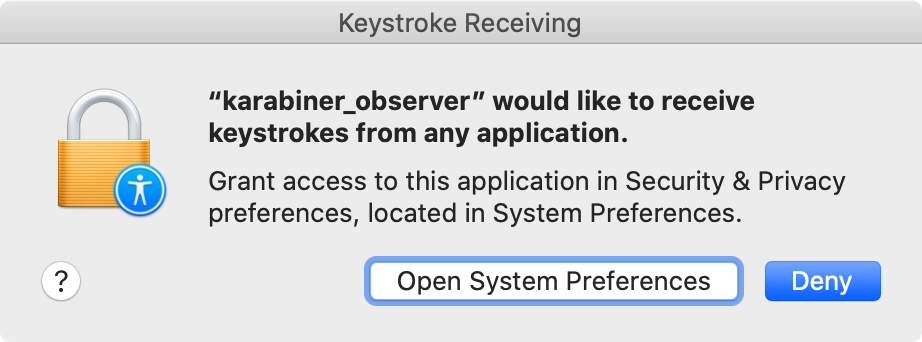
\includegraphics[scale=0.35]{fig/Karabiner_keystroke.png}
  \caption{Karabiner-Elementsのキーボード入力への警告}
  \label{fig:Karabiner_keystroke}
\end{figure}

このダイアログに従い「Open System Preferences」をクリックすると、図~\ref{fig:Karabiner_privacy}が現れます。ここで再び鍵アイコンを解錠し、Karabiner-Elements関係のファイルがキーボード入力を読み取れるように許可を出します。

\begin{figure}
  \centering
  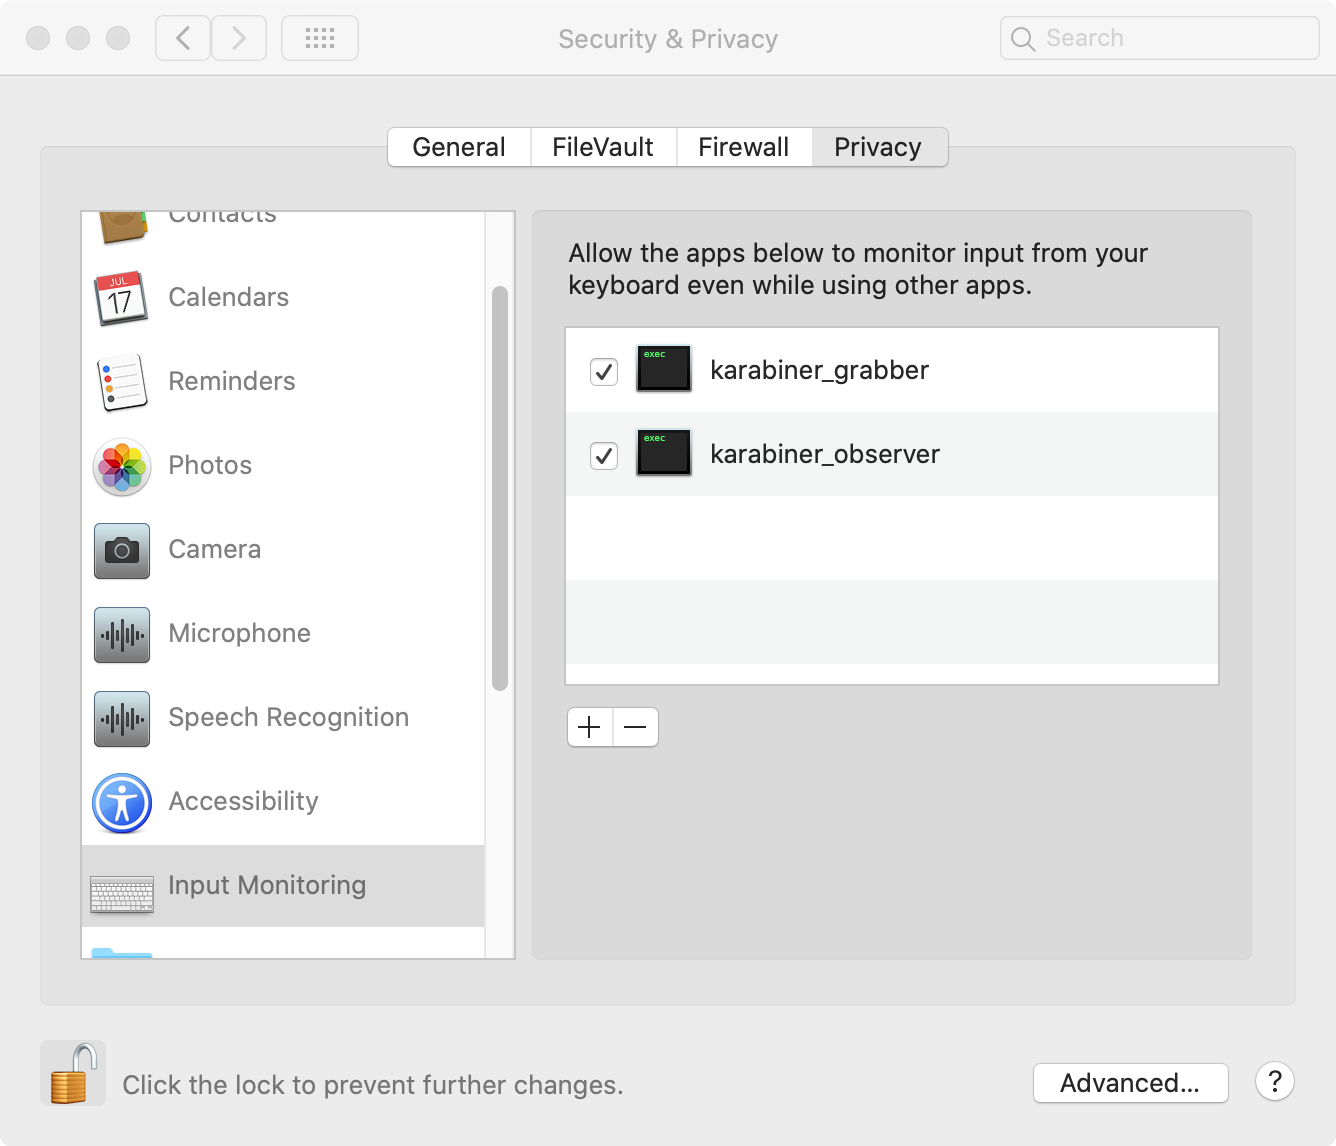
\includegraphics[scale=0.35]{fig/Karabiner_privacy.png}
  \caption{Karabiner-Elementsのプライバシー設定}
  \label{fig:Karabiner_privacy}
\end{figure}

さて、これでようやくKarabiner-Elementsが使用できます。USキーボードを使用している場合は、まず図~\ref{fig:Karabiner_simple}のように「Simple modifications」のタブでCaps LockキーをControlキーに変更してください。

\begin{figure}
  \centering
  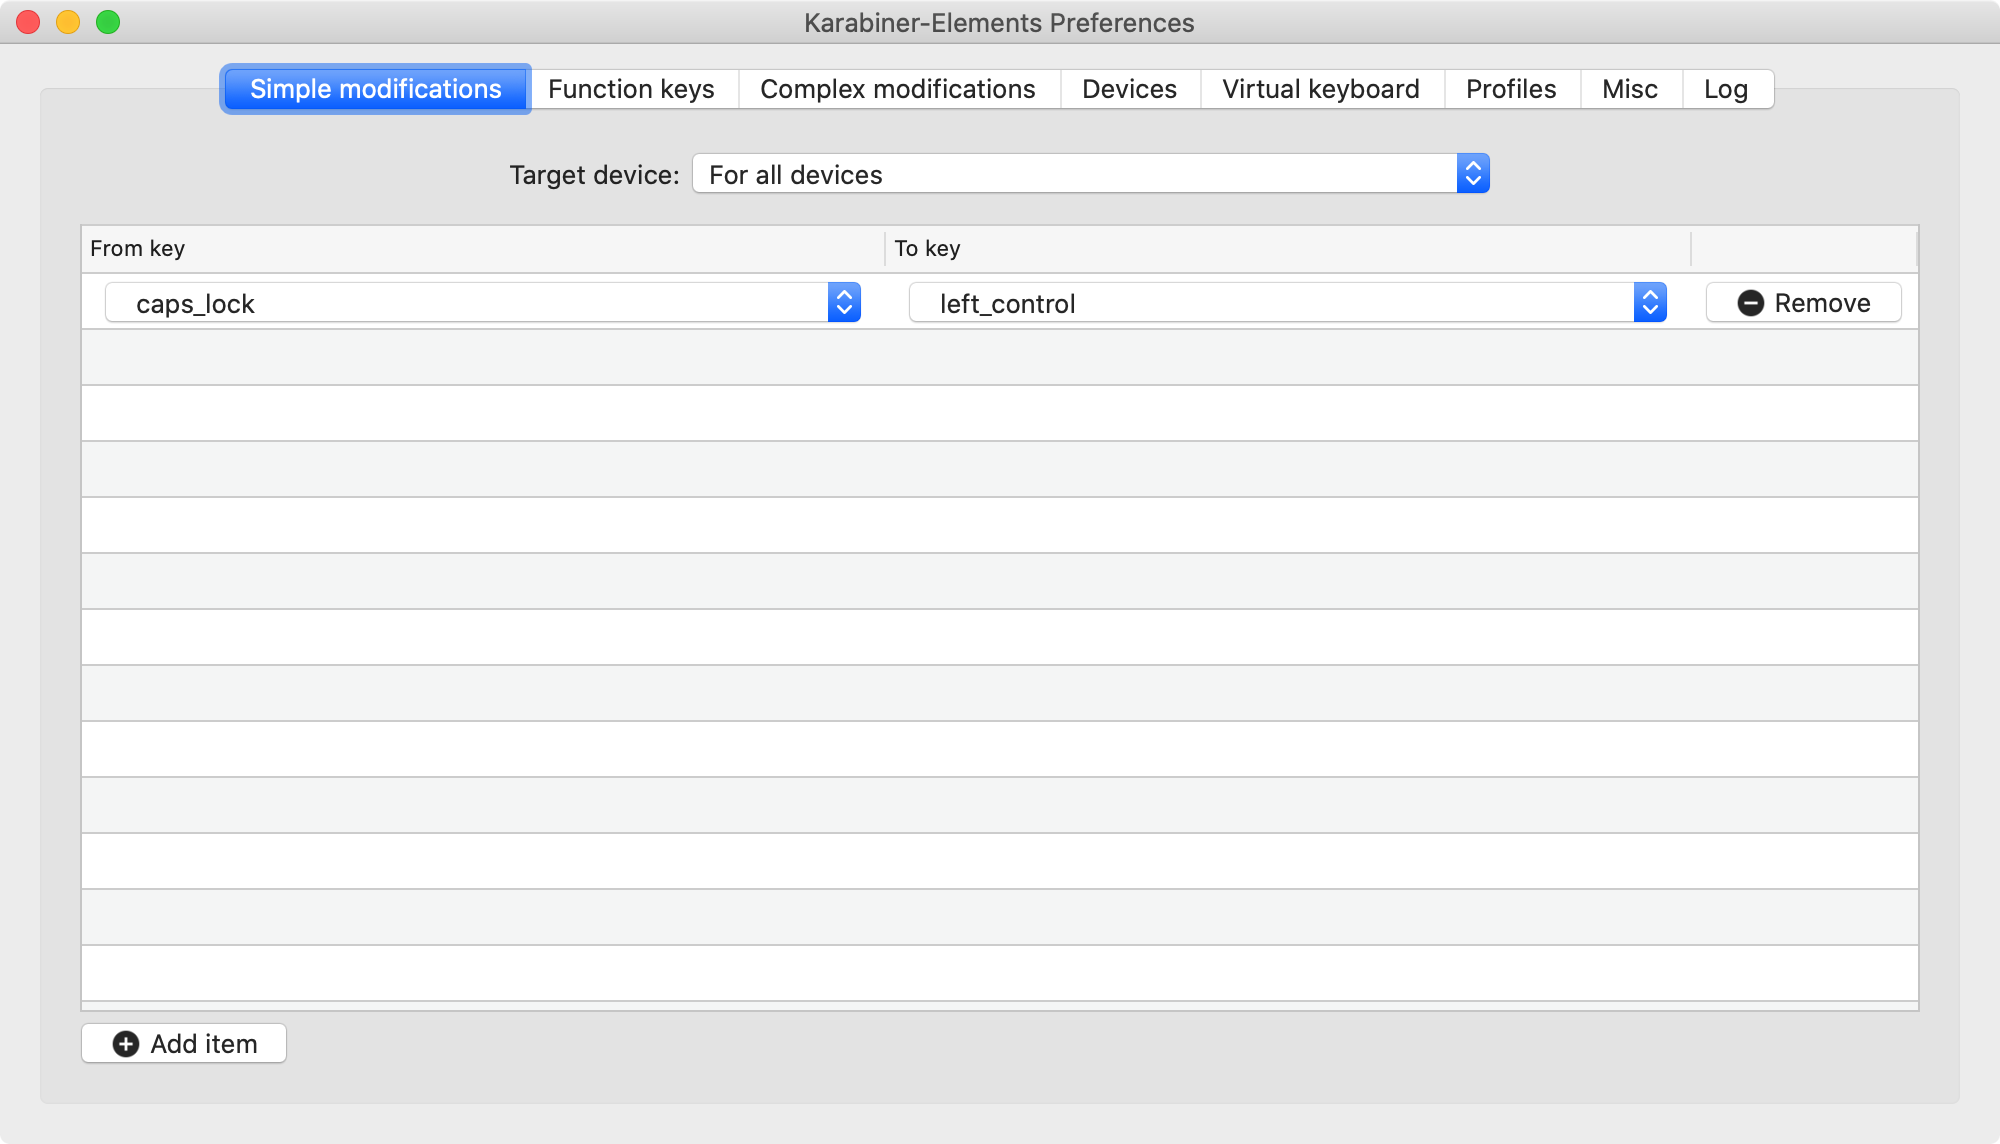
\includegraphics[scale=0.35]{fig/Karabiner_simple.png}
  \caption{Karabiner-Elementsの設定画面}
  \label{fig:Karabiner_simple}
\end{figure}

次に図~\ref{fig:Karabiner_import}のように「Complex modifications」タブから「Add rule」クリックし、「Import more rules from the Internet」を押してください。様々なキーボード動作の設定がダウンロードできるので、「Emacs key bindings (rev 12)」をダウンロードしましょう。USキーボードの場合は「For Japanese (日本語環境向けの設定) (rev 5)」も追加します。

\begin{figure}
  \centering
  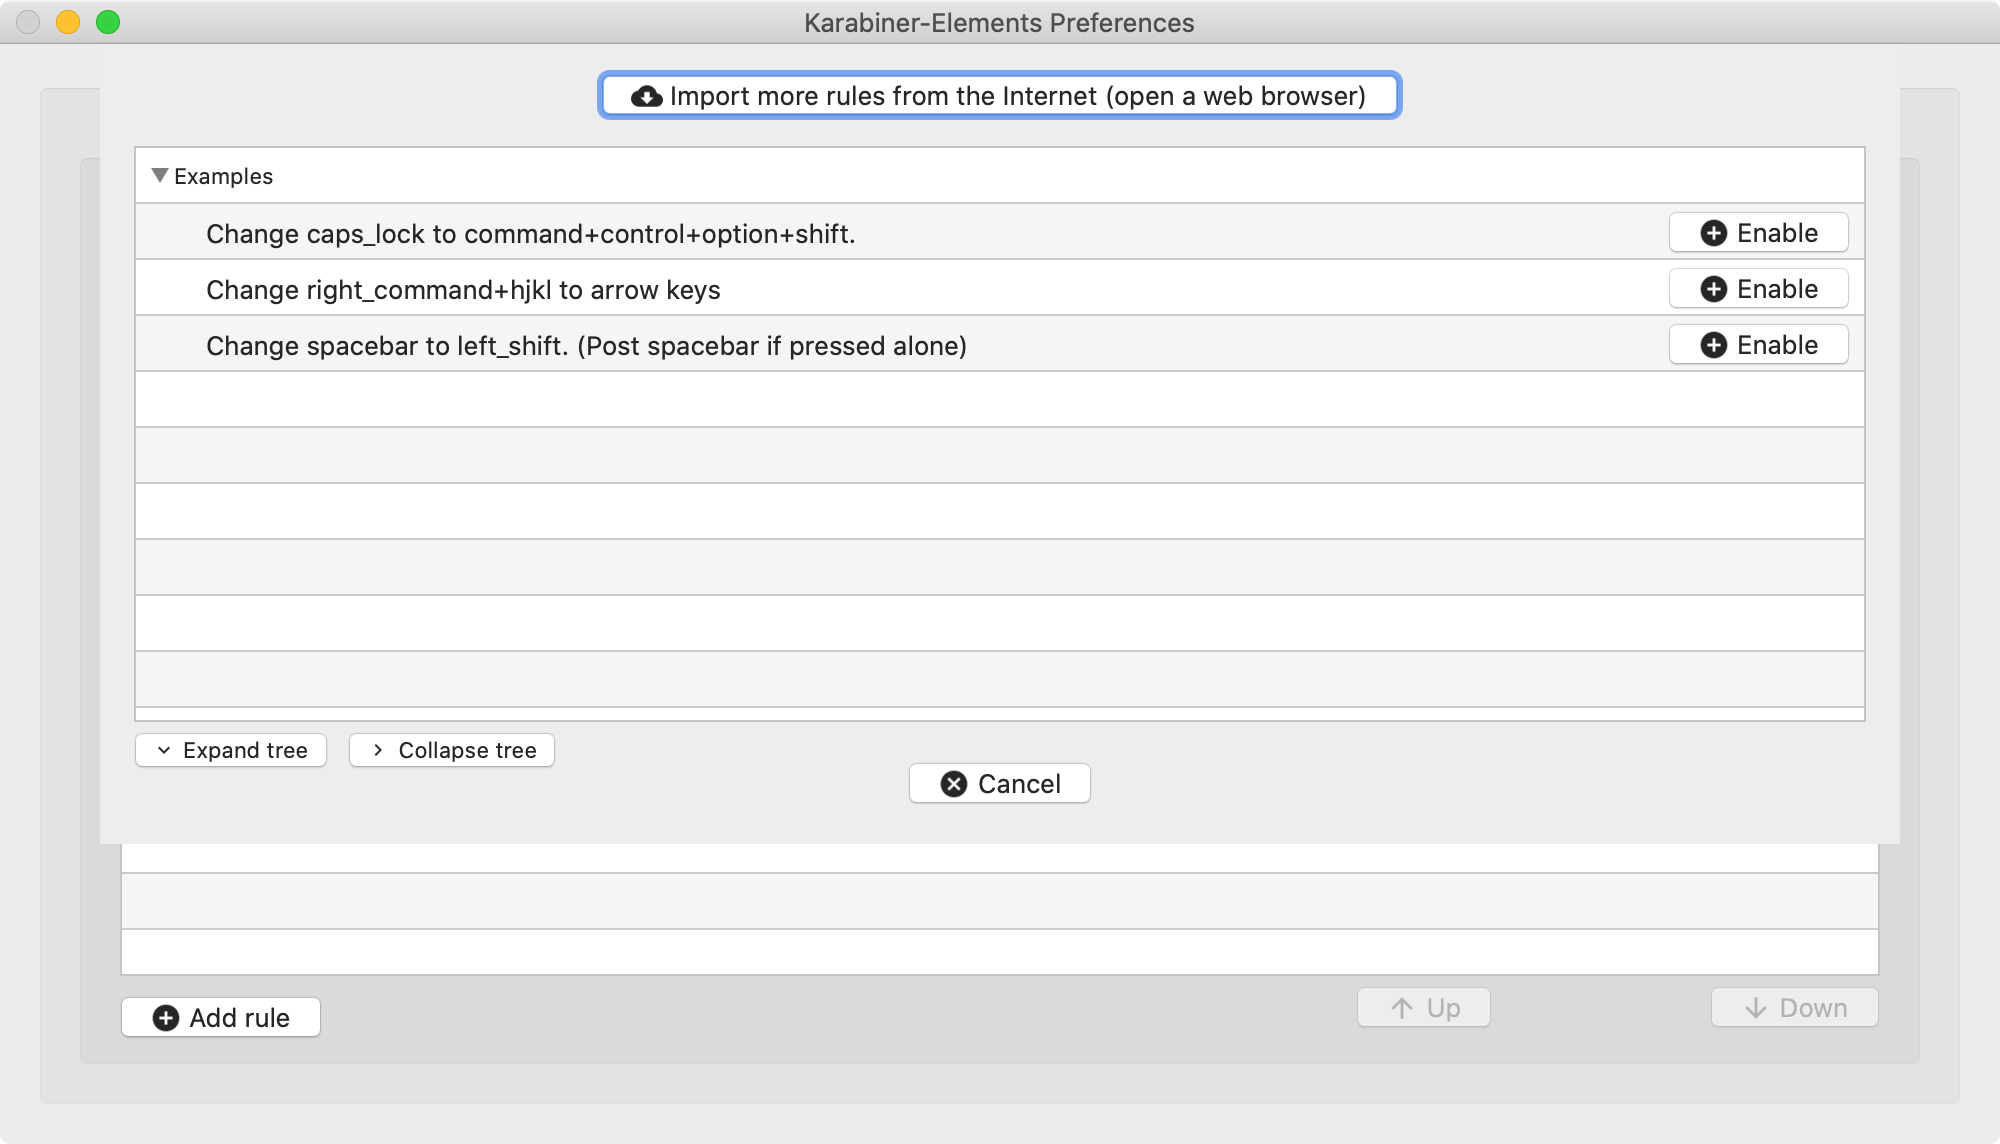
\includegraphics[scale=0.35]{fig/Karabiner_import.png}
  \caption{Karabiner-Elementsの設定のインポート}
  \label{fig:Karabiner_import}
\end{figure}

最後に「Emacs key bindings [control+keys] (rev 10)」を「Enable」にします。USキーボードの場合は「コマンドキーを単体で押したときに、英数・かなキーを送信する。(左コマンドキーは英数、右コマンドキーはかな) (rev 3)」も追加します。

\section{Emacsの操作体系に慣れる}
\label{sec:Emacs}

ここでは、macOSでの標準的なエディタ(editor)のひとつであるEmacsの操作について、その初歩の初歩について説明します\footnote{macOS Mojaveまでは\texttt{/usr/bin/emacs}が最初からインストールされていましたが、Catalinaからはなくなりました。GNUライセンスで配布されているソフトウェアの使用を回避するためと言われています。代わりに\texttt{/usr/bin/mg}というEmacsに似たエディタ(Emacsクローン)がインストールされています。}。エディタは文章を書くためのソフトウェアです。ただし、ワープロのように様々な装飾をするための機能はありません。プログラムを書いたり、\LaTeX{}のソースを書いたりと、装飾ではなく文そのものに意味があるときに使います。そのような作業に特化したワープロにはない様々な機能が搭載されています。

Emacsの特徴のひとつに、文字入力に特殊なキーボードショートカット(Emacs key binding)を使うことが挙げられます。慣れないうちは全く便利に感じないと思いますが、一度慣れてしまうと、もう他のエディタには戻れなくなるのでぜひ覚えて下さい。macOSを使う場合、このショートカットをほとんどのソフトウェアでも利用可能です。基本的なキーボードショートカットの一覧を表\ref{tab_emacs}にまとめました。

\begin{table}
  \centering
  \caption{Emacsの基本的なキーボードショートカット}
  \label{tab_emacs}
  \begin{tabular}{llp{10cm}}
  \hline
ショートカット & 英単語 & 機能 \\ \hline\hline
C-f & {\bf F}orward & 一文字進む(→キーと同等) \\
C-b & {\bf B}ackward & 一文字戻る(←キーと同等) \\
C-p & {\bf P}revious line & 次の行へ進む(↓キーと同等) \\
C-n & {\bf N}ext line & 前の行へ戻る(↑キーと同等) \\
C-a & {\bf A}head & 行頭へ移動 \\
C-e & {\bf E}nd & 行末へ移動 \\
C-k & {\bf K}ill & カーソル位置から行末までを全て kill-ring と呼ばれるメモリ領域に移動(カットに類似) \\
C-y & {\bf Y}ank & kill-ringにあるものをカーソル位置にペースト \\
C-t & {\bf T}ranspose & カーソルの前後の文字を入れ替える \\
C-h & 不明 & カーソル前方を一文字削除(MacのDelete、WindowsのBackspaceと同等) \\
C-d & forward {\bf D}elete & カーソル後方を一文字削除(WindowsのDeleteと同等) \\
C-m & 不明 & 改行(カーソルも次の行へ移動する) \\
C-o & 不明 & 改行(カーソルは元の位置にとどまる) \\
C-Space C-w & 不明 & C-Space入力時のカーソル位置から、C-w入力時のカーソル位置までの範囲をkill-ringに移動する \\ \hline
C-x C-f & {\bf F}ind file & 既存ファイルを開く、なければ作成する \\
C-x C-s & {\bf S}ave & ファイルを保存する \\
C-x C-c & 不明 & 終了する \\
C-x C-w & 不明 & ファイルを別名で保存する \\
C-x C-2 & 不明 & ウインドウを二分割にする \\
C-x C-1 & 不明 & ウインドウを一分割にする \\
C-s & {\bf S}earch & 検索する \\
C-r & {\bf R}verse search & 後方に検索する \\
M gg & 不明 & 特定の行に移動する\\\hline
  \end{tabular}
\end{table}

\ref{sec:Homebrew}章を参考にして、まずはEmacsをインストールしてみてください。\texttt{Emacs}というコマンドを設定し終えたところまでを想定します。

次のコマンドで、Emacsを立ち上げます。図~\ref{fig:Emacs}のような画面が現れるはずです。
\begin{lstlisting}[language=bash]
$ Emacs
\end{lstlisting}

\begin{figure}
  \centering
  \subfigure[]{
    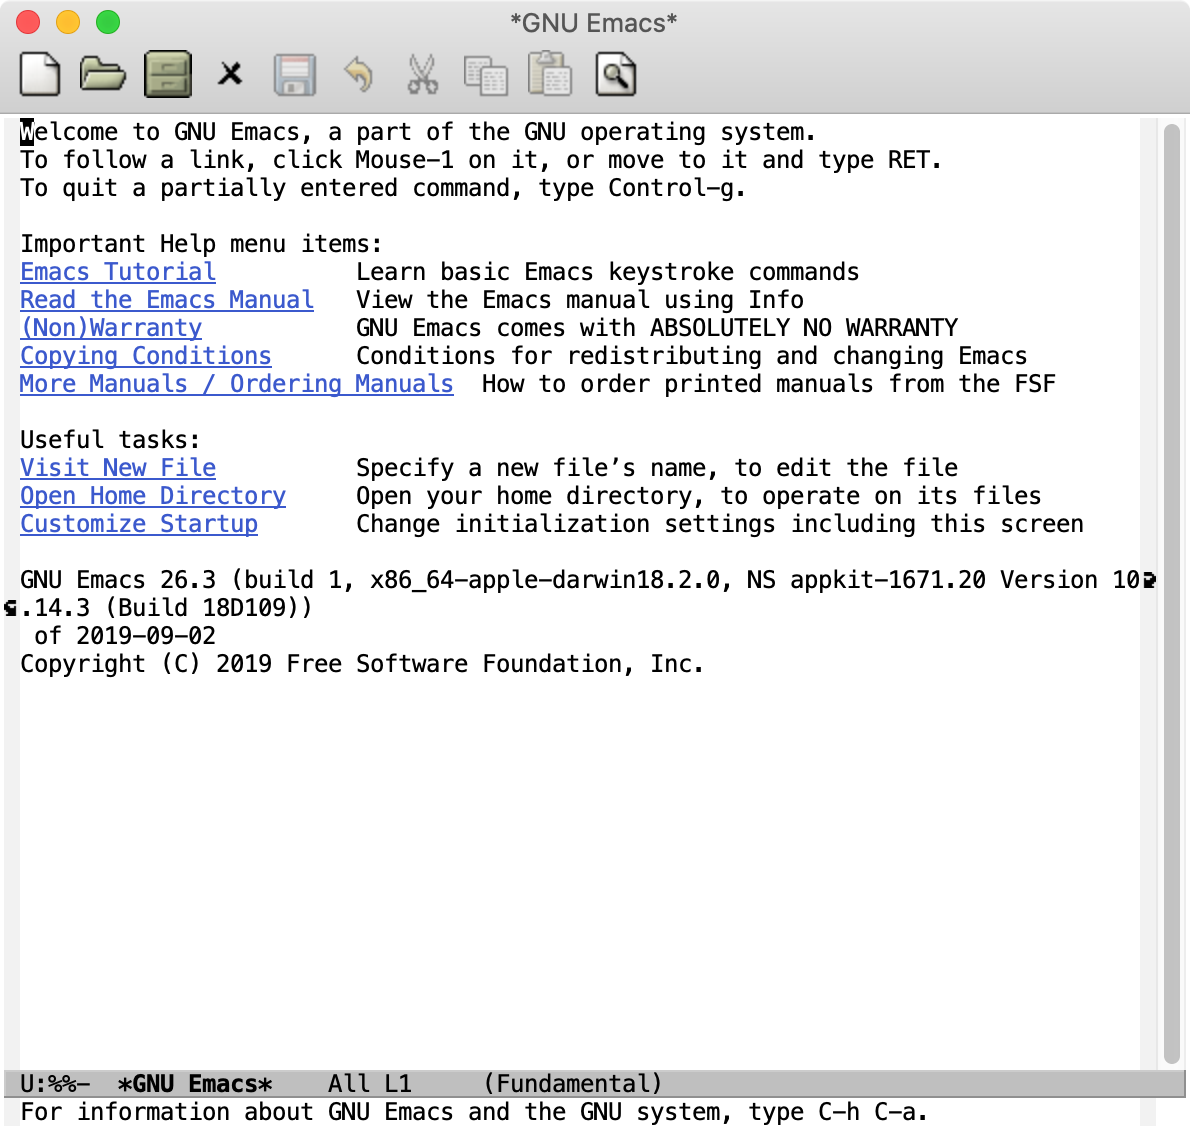
\includegraphics[width=.32\textwidth,clip]{fig/Emacs.png}%
    \label{fig:Emacs}%
  }\hfill%
  \subfigure[]{%
    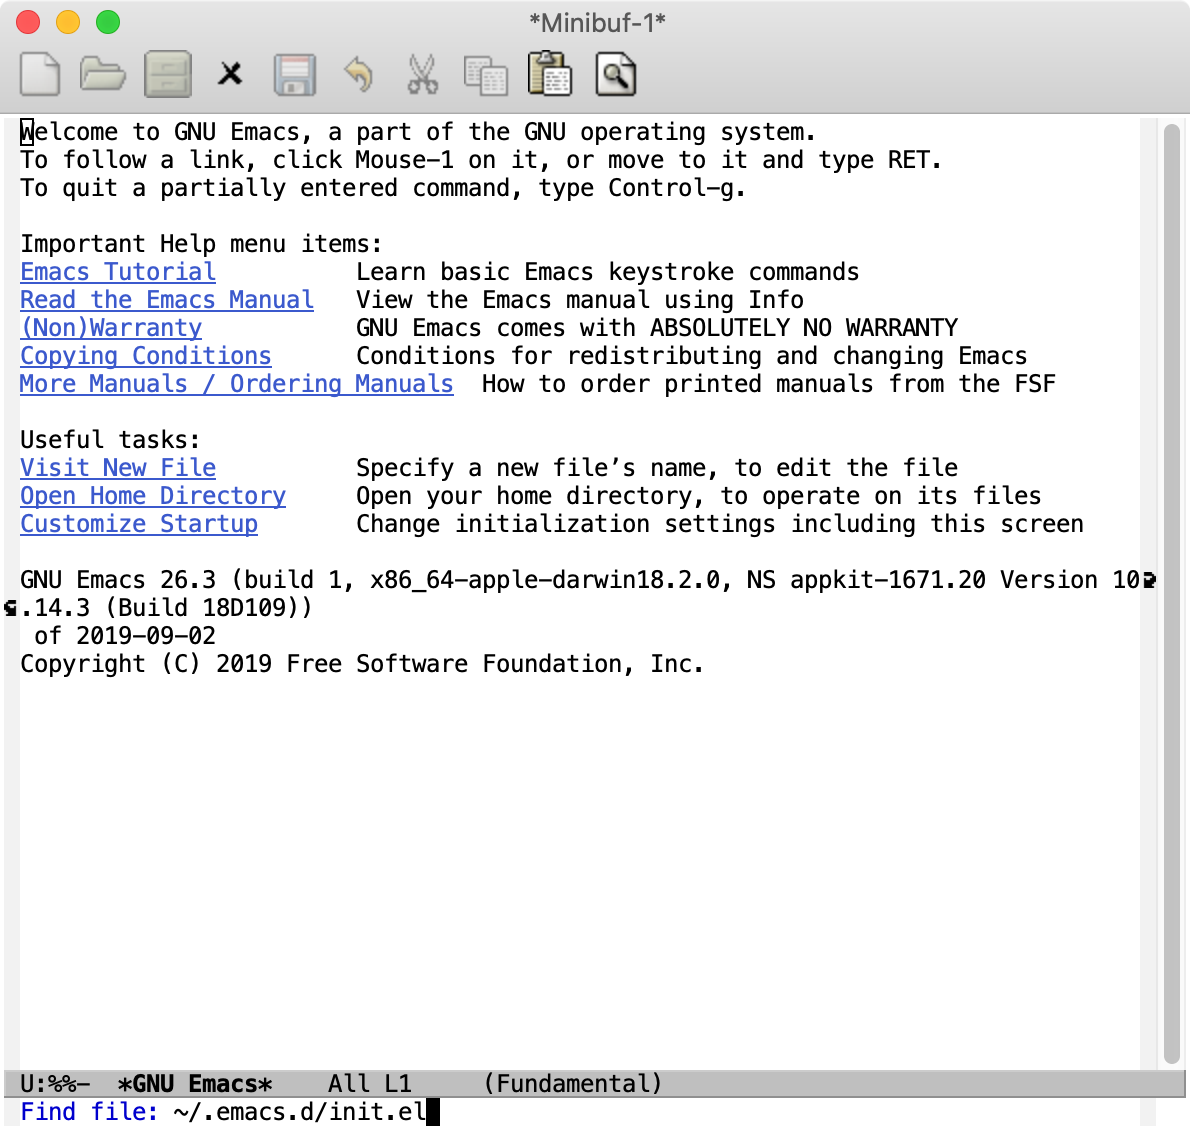
\includegraphics[width=.32\textwidth,clip]{fig/Emacs_CxCf.png}%
    \label{fig:Emacs_CxCf}%
  }\hfill%
  \subfigure[]{%
    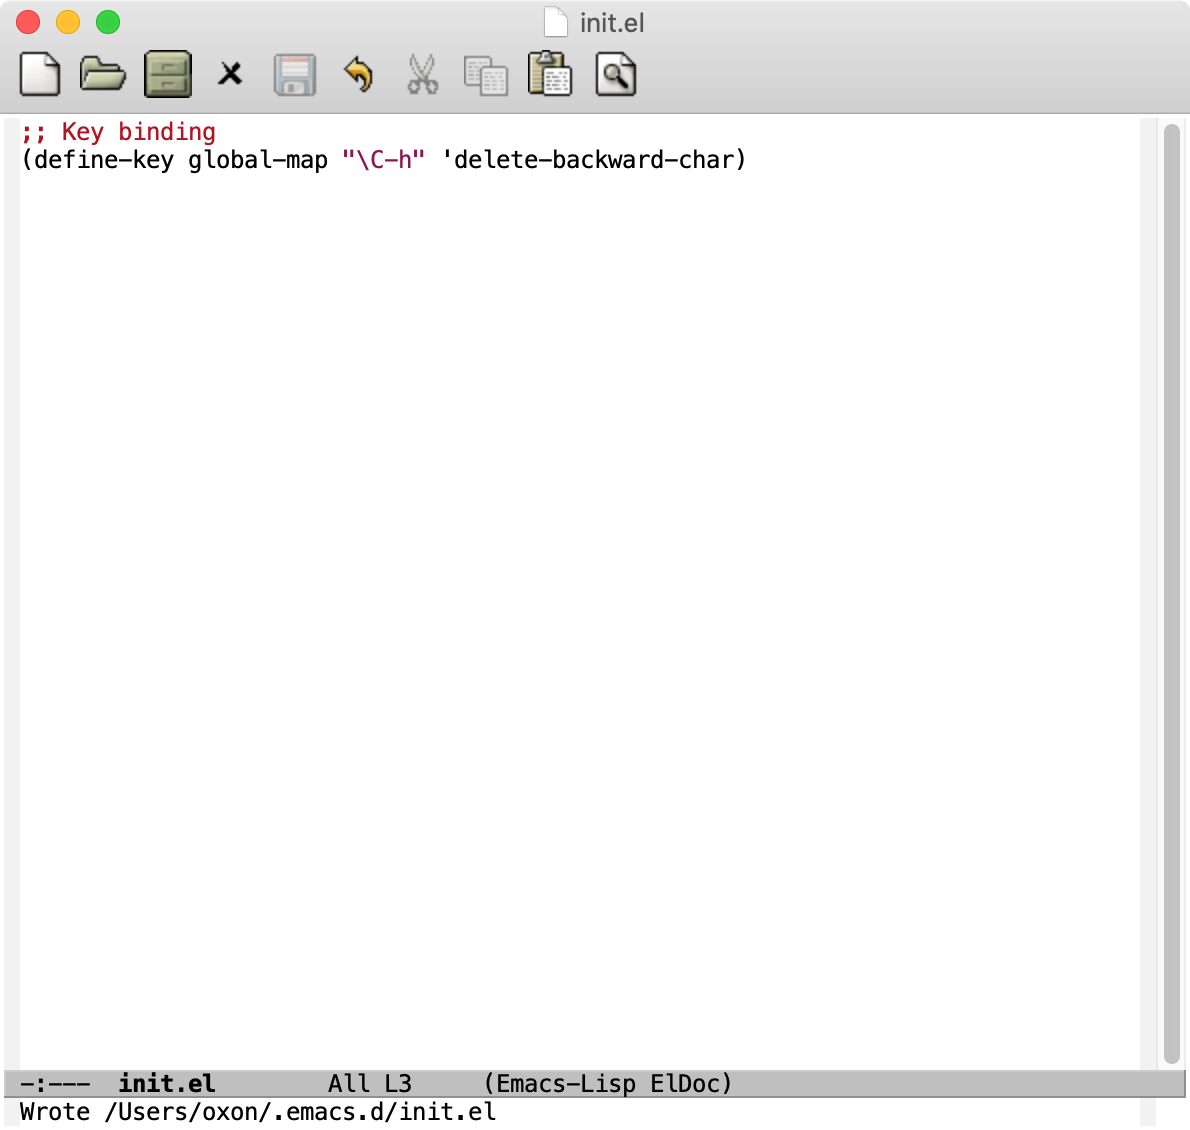
\includegraphics[width=.32\textwidth,clip]{fig/Emacs_CxCs.png}%
    \label{fig:Emacs_CxCs}
  }
  \caption{Emacsの起動画面 (a) Emacsを立ち上げたところ。(b) \texttt{C-x C-f}で\texttt{\~{}/.emacs.d/init.el}を新規作成するところ。(c) 編集後に\texttt{C-x C-s}で保存したときの画面。}
\end{figure}

まずは、新しいファイルを作成してみましょう。最初に作成するのは、Emacsの設定ファイルです。図~\ref{fig:Emacs}の状態から、Controlキー\footnote{USキーボードでCaps LockキーをControlキーに変更した場合は、そのキー。}を左手小指で押しっぱなしにし、左手中指でXキーを同時に押します。その後Xキーから薬指を離し、Controlキーは押した状態のまま左手人さし指でFキーを同時に押します。これを、「C-x C-f」のように表記します\footnote{Control-x、Ctl-x、Cn-xなど、いくつかの表記方法があります。好みの問題です。}。表\ref{tab_emacs}にあるように、これは新規ファイルを作成するためのショートカットです。図\ref{fig:Emacs_CxCf}のように一番下の「Find file:」の後に続けて作成したいファイル名を入力し、リターンきーを押しましょう。ここでは\texttt{\~{}/.emacs.d/init.el}を作成しています\footnote{これは、ホームディレクトリの中にある不可視ディレクトリ\texttt{.emacs.d}の中にある\texttt{init.el}というファイルの意味です。}。

そのファイルが存在しない場合は、新規作成されます。真っ白な画面に切り替わったら、次の内容を入力します。
\begin{lstlisting}[language=lisp]
;; Key binding
(define-key global-map "\C-h" 'delete-backward-char)
\end{lstlisting}
そして、\texttt{C-x C-s}で編集内容を保存すると、図~\ref{fig:Emacs_CxCs}のようになるはずです。最後に、\texttt{C-x C-c}でEmacsを終了します。ここで追加した設定は、1行目はただのコメント(なくても動作は変わりません)、2行目は\texttt{C-h}を1文字削除の動作に変更するための設定です。

Emacsの操作に慣れるには、まずこのControlキーを多用した操作に慣れることが重要です。表\ref{tab_emacs}に挙げたショートカットを中心にまずは覚え、どのような操作や機能、設定があるのかを調べていきましょう。多機能過ぎて、うんざりするはずです。

\section{C-Space C-wをmacOSで使う}

表\ref{tab_emacs}に示したショートカットの多くはmacOSのアプリケーションでも使うことができます。また使えないアプリケーションでも、\ref{sec:Karabiner}に書いたようにKarabiner-Elementsの設定で使用可能になります。

例えばKarabiner-Elementsで\texttt{C-p}や\texttt{C-f}を有効にしておくと、Finderのカラム表示での移動が非常に早く、楽になります。

しかしmacOSのデフォルトの状態では\texttt{C-Space C-w}はmacOSのアプリケーションでは使うことができません。Emacsに慣れてくると、\texttt{C-Space C-w}がEmacs以外で使えないのが不便に感じるでしょう。macOSにはこの操作を実現するための機能が隠されています。

コード\ref{code:DefaultKeyBinding}を、\texttt{\~{}/Library/KeyBindings/DefaultKeyBinding.dict}として保存して下さい\footnote{\url{https://developer.apple.com/library/archive/documentation/Cocoa/Conceptual/EventOverview/TextDefaultsBindings/TextDefaultsBindings.html}に詳しい解説がある。}。「Mail」などを起動して文字入力する際に、\texttt{C-Space C-w}や\texttt{C-x C-s}が有効になっているはずです。

%\begin{NoFloat}
\lstinputlisting[float=tb,caption=\texttt{DefaultKeyBinding.dict},label=code:DefaultKeyBinding,numbers=left]{src/DefaultKeyBinding.dict}
%\end{NoFloat}

\section{Xcode}

\begin{lstlisting}[language=bash]
$ clang
xcode-select: note: no developer tools were found at '/Applications/Xcode.app', requesting install. Choose an option in the dialog to download the command line developer tools.
\end{lstlisting}

\begin{figure}
  \centering
  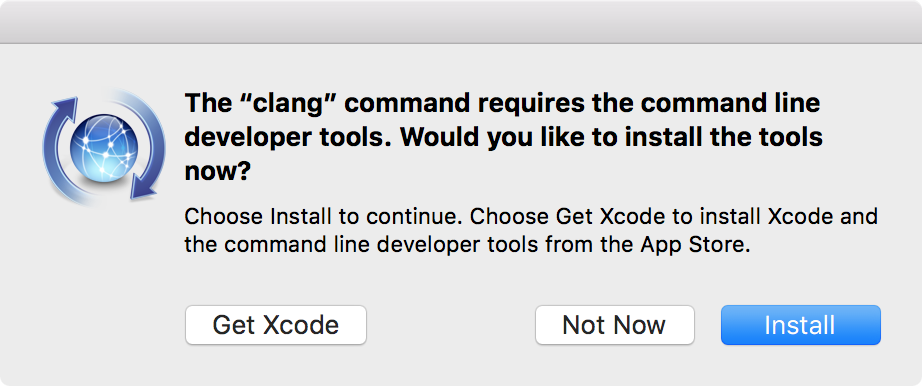
\includegraphics[scale=0.5]{fig/command-line-developer-tools.png}
  \caption{Command Line Developer Tools のインストールダイアログ}
  \label{fig:command-line-developer-tools}
\end{figure}

\begin{lstlisting}[language=bash]
$ clang
clang: error: no input files
\end{lstlisting}

\section{知っていると便利な macOS 特有のコマンド}

\chapter{configure と Make}
\label{chap:configure}

\section{\texttt{configure}を使った ROOT のコンパイル(非推奨)}
\label{sec:compile_configure}

最近のROOTでは非推奨もしくは全くサポートされていません\footnote{少なくとも6.16/00以降ではサポートされていません。}が、\texttt{configure}スクリプトと\texttt{make}コマンドを使ったROOTのビルドは、かつて標準的な手法でした。また同様の手法で多くのオープンソースソフトウェアをビルドすることもできますので、ここでは参考として\texttt{configure}と\texttt{make}を使ったビルド方法を紹介します。

まずは\texttt{CMake}の時と同様にROOTのソースコードを\texttt{/usr/local}に展開します。
\begin{lstlisting}[language=bash]
$ cd /usr/local
$ sudo tar zxvf ~/root_v6.12.06.source.tar.gz
\end{lstlisting}

次に\texttt{configure}スクリプトを実行します。このスクリプトは\texttt{CMake}や\texttt{CmakeLists.txt}と同様に、ソフトウェアのビルドに必要な情報を集約します。

\begin{lstlisting}[language=bash]
$ cd root-6.12.06
$ sudo ./configure
\end{lstlisting}

色々とターミナルに出力されますが、最後に次のような表示が出れば\texttt{configure}は成功です。もし何かしらのエラーが表示される場合、ROOTのビルドに必要な他のコマンドやライブラリがインストールされていないことが考えられます。表示されたエラーをよく読み、原因が何かを考えて対応しましょう。
\begin{lstlisting}[language=bash]
Enabled support for asimage, astiff, bonjour, builtin_afterimage, builtin_ftgl, builtin_freetype, builtin_gl2ps, builtin_glew, builtin_unuran, builtin_lz4, builtin_llvm, libcxx, cocoa, explicitlink, fink, fitsio, gviz, genvector, krb5, ldap, memstat, opengl, python, rpath, search_usrlocal, shared, sqlite, tmva, xml.

To build ROOT type:

   make 

******************************************************************************
* The classic configure/make method of building ROOT is now DEPRECATED in    *
* favor of the CMake one.                                                    *
* Refer to README/INSTALL file for updated instructions or visit the page    *
* https://root.cern.ch/building-root                                         *
******************************************************************************
\end{lstlisting}
6.12/06では、\texttt{configure}を使ったビルドは「DEPRECATED」(旧式で非推奨)であると表示されます。新しいROOTを使う場合は、節~\ref{subsec:compile_cmake}の\texttt{CMake}を使ったビルドを推奨します。

あとは、\texttt{CMake}のときと同様に\texttt{make}を実行します。
\begin{lstlisting}[language=bash]
$ sudo make -j8
\end{lstlisting}
うまくコンパイルが全て完了すると、次のような表示が最後に出るはずです。
\begin{lstlisting}
root [0] 
Processing hsimple.C...
hsimple   : Real Time =   0.07 seconds Cpu Time =   0.05 seconds
(TFile *) 0x7fb0fae560c0
 
   ============================================================
   ===                ROOT BUILD SUCCESSFUL.                ===
   === Run 'source bin/thisroot.[c]sh' before starting ROOT ===
   ============================================================
\end{lstlisting}

\texttt{make}実行時に何もオプションを渡さない場合、発展的な機能やマイナーな機能は「Enabled support」の一覧に入りません。\texttt{make}実行時に例えば次のようにオプションをつけることで、オプションもビルドすることができるようになります。

\begin{lstlisting}[language=bash]
$ sudo ./configure --enable-minuit2 --enable-gdml
\end{lstlisting}

\texttt{configure}を使った場合は展開したソースファイルのディレクトリ内でコンパイルを行いますので、次のような\texttt{\~{}/.bashrc}の設定になります。
\begin{NoFloat}
\lstinputlisting[language=bash]{src/bashrc.sh}
\end{NoFloat}

\section{configureとMakeの一般的な解説}

macOSやLinux環境でソフトウェアを導入する時、インストールの方法は主に3つあります。1つ目は、\ref{sec:Homebrew}で説明したようなパッケージ管理ソフト\footnote{macOSではMacPorts、Fink、Homebrewなど、LinuxではYumやAPTなど。}を使う方法す。2つ目は、既にコンパイル済みでバイナリ配布されているソフトを導入する方法です。例えば、KeyRemap4MacBookをインストーラを使ってインストールしたのがこれに当たります。また、ROOTを入れる場合でもバイナリ配布されているものを使うことが可能です。3つ目は、ソースコードの配布されているソフトウェアを自分でコンパイル(compile)する\footnote{ビルド(build)するとも言います。}方法です。これは\ref{sec:ROOT_install}でROOTの導入として説明しました。

自分でソフトウェアをソースコードからコンパイルする場合、標準的なやり方が存在します。また、研究で通常使うソフトウェアの多くがこの標準的な方法に則して作成されています。そのためここで説明する方法を覚えておけば、多くのソフトウェアを自分で簡単にインストールできるようになります。

このやり方を覚えるために、「GNU Hello\footnote{\url{http://www.gnu.org/software/hello/}}」と呼ばれるソフトウェアを試しにインストールしてみましょう。この「GNU Hello」は標準的な方法を学ぶ上で最適なもので、インストールしても実用性はありません。

まず、次のコマンドで\url{http://ftp.gnu.org/gnu/hello/}から最新版の\texttt{hello-2.8.tar.gz}を落としてきて展開します。展開されたディレクトリに移動して\texttt{ls}で中身を見てみましょう。

\begin{lstlisting}[language=bash]
$ curl -O http://ftp.gnu.org/gnu/hello/hello-2.8.tar.gz
  % Total    % Received % Xferd  Average Speed   Time    Time     Time  Current
                                 Dload  Upload   Total   Spent    Left  Speed
100  681k  100  681k    0     0   150k      0  0:00:04  0:00:04 --:--:--  166k
$ tar zxf hello-2.8.tar.gz
$ cd hello-2.8 
$ ls
ABOUT-NLS      INSTALL        THANKS         configure.ac   man
AUTHORS        Makefile.am    TODO           contrib        po
COPYING        Makefile.in    aclocal.m4     doc            src
ChangeLog      NEWS           build-aux      lib            tests
ChangeLog.O    README         config.in      m4
GNUmakefile    README-release configure      maint.mk
\end{lstlisting}

ここで重要なのは、\texttt{README}、\texttt{INSTALL}、\texttt{configure}の3つです。\texttt{README}は、そのソフトウェアに関する全般的な説明が書かれています。\texttt{INSTALL}には、そのソフトウェアのインストール方法が書かれています。\texttt{less}コマンドなどで、試しに中身を読んでみて下さい。

\begin{lstlisting}[language=bash]
$ less README
$ less INSTALL
\end{lstlisting}

\texttt{configure}はシェルスクリプトで、そのソフトウェアをコンパイルするときに必要なライブラリやコマンドが存在するかどうか、存在するパスはどこか、OSの環境は何かを自動的に調べて必要な設定をしてくれます。また、必要に応じてユーザが様々なオプションを指定することができます。どのようなオプションがあるかは、次のようにヘルプを表示することで読むことができます。

\begin{lstlisting}[language=bash]
$ ./configure --help
\end{lstlisting}

様々なオプションが表示されますが、このうち最も頻繁に使われるのがインストール先の指定のオプション\texttt{--prefix}です。次のように\texttt{configure}を実行することで、\texttt{hello}コマンドを\texttt{/usr/local/bin}にインストールし、またマニュアルを\texttt{/usr/local/share/man/man1}にインストールします。もし\texttt{/usr/local}の代わりに他の場所をしていすれば、これらのファイルは指定した場所の下にインストールされます。
\begin{lstlisting}[language=bash]
$ ./configure --prefix=/usr/local
\end{lstlisting} 

\texttt{configure}が問題なく実行されれば、\texttt{Makefile}というファイルが新たに生成されているはずです。このファイルの中には、そのソフトウェアをどのような手順でコンパイルすれば良いかが全て書かれています。ユーザはどのようなソースコードがあるのかなどを気にする必要はありません。この\texttt{Makefile}の手順の通りに自動的にソフトウェアをコンパイルするには、以下の
コマンドを打つだけです。

\begin{lstlisting}[language=bash]
$ make -j 4
\end{lstlisting} 

\texttt{make}コマンドが\texttt{Makefile}の中身を自動的に調べ、そこに書かれている手順を追ってコンパイルを行います。\texttt{-j 4}のオプションは、使っているCPU能力を最大限に引き出すためのものです。この場合、4コアのCPUを全て使ってくれます。

これで必要なファイルが全て生成されたので、最後にインストール作業を行います。通常は\texttt{/usr/local}にインストールする場合に管理者権限が必要なので、次のコマンドを実行します。

\begin{lstlisting}[language=bash]
$ sudo make install
Password:
\end{lstlisting}

これで、\texttt{/usr/local/bin/hello}などが配置されたはずです。では、確認のため\texttt{hello}を実行しましょう。 
\begin{lstlisting}[language=bash]
$ hello
Hello, world!
\end{lstlisting}

どのようなオプションを渡せるかは、\texttt{--help}や\texttt{-h}をつけて確認します。
\begin{lstlisting}[language=bash]
$ hello -h
Usage: hello [OPTION]...
Print a friendly, customizable greeting.

  -h, --help          display this help and exit
  -v, --version       display version information and exit

  -t, --traditional       use traditional greeting format
  -n, --next-generation   use next-generation greeting format
  -g, --greeting=TEXT     use TEXT as the greeting message

Report bugs to: bug-hello@gnu.org
GNU Hello home page: <http://www.gnu.org/software/hello/>
General help using GNU software: <http://www.gnu.org/gethelp/>
\end{lstlisting}

また\texttt{hello}コマンドのマニュアルを見るには\texttt{man}コマンドを使います。

\begin{lstlisting}[language=bash]
$ man hello
\end{lstlisting}

\chapter{本文で登場したROOTスクリプトのPyROOT版}
ここでは、本文中で登場したROOTスクリプトをPyROOTで書き換えた例を掲載します。\texttt{foo.C}というROOTスクリプトであれば、\texttt{foo.py}というPyROOTスクリプトにしてあります。

\begin{NoFloat}
\lstinputlisting[language=python,breaklines=true,caption=\texttt{population.py},label=code:population_py,numbers=left]{src/population.py}
\end{NoFloat}
